% !TeX encoding = UTF-8
% !TeX program = pdflatex
% !TeX spellcheck = en_US

\documentclass[LaM,binding=0.6cm]{sapthesis}

\linespread{1.2}

\usepackage{microtype}

\usepackage{hyperref}
\hypersetup{pdftitle={Planning and Executing Humanoid Gaits
  in a World of Stairs},pdfauthor={Michele Cipriano}}

% Remove in a normal thesis
\usepackage{lipsum}
\usepackage{curve2e}
\definecolor{gray}{gray}{0.4}
\newcommand{\bs}{\textbackslash}

% Algorithms:
\usepackage[ruled,vlined,linesnumbered]{algorithm2e}

% Math symbols:
%%%%%%% Mathematical Symbols ==>>

\def\tr{^T}
\def\trd{{}^T}
\def\Atan{\mathrm{Atan2}}
\def\Acos{\mathrm{Acos}}
\def\sgn{\mathrm{sgn}}
\def\de{\mathrm{d}}
\def\diag{\mathrm{diag}}

\def\zero{\hbox{\bf 0}}
\def\Zero{{\mbox{\boldmath $O$}}}

\def\bfa{{\mbox{\boldmath $a$}}}
\def\bfb{{\mbox{\boldmath $b$}}}
\def\bfc{{\mbox{\boldmath $c$}}}
\def\bfd{{\mbox{\boldmath $d$}}}
\def\bfe{{\mbox{\boldmath $e$}}}
\def\bff{{\mbox{\boldmath $f$}}}
\def\bfg{{\mbox{\boldmath $g$}}}
\def\bfh{{\mbox{\boldmath $h$}}}
\def\bfi{{\mbox{\boldmath $i$}}}
\def\bfj{{\mbox{\boldmath $j$}}}
\def\bfk{{\mbox{\boldmath $k$}}}
\def\bfl{{\mbox{\boldmath $l$}}}
\def\bfm{{\mbox{\boldmath $m$}}}
\def\bfn{{\mbox{\boldmath $n$}}}
\def\bfo{{\mbox{\boldmath $o$}}}
\def\bfp{{\mbox{\boldmath $p$}}}
\def\bfq{{\mbox{\boldmath $q$}}}
\def\bfr{{\mbox{\boldmath $r$}}}
\def\bfs{{\mbox{\boldmath $s$}}}
\def\bft{{\mbox{\boldmath $t$}}}
\def\bfu{{\mbox{\boldmath $u$}}}
\def\bfv{{\mbox{\boldmath $v$}}}
\def\bfw{{\mbox{\boldmath $w$}}}
\def\bfx{{\mbox{\boldmath $x$}}}
\def\bfy{{\mbox{\boldmath $y$}}}
\def\bfz{{\mbox{\boldmath $z$}}}
\def\bfA{{\mbox{\boldmath $A$}}}
\def\bfB{{\mbox{\boldmath $B$}}}
\def\bfC{{\mbox{\boldmath $C$}}}
\def\bfD{{\mbox{\boldmath $D$}}}
\def\bfE{{\mbox{\boldmath $E$}}}
\def\bfF{{\mbox{\boldmath $F$}}}
\def\bfG{{\mbox{\boldmath $G$}}}
\def\bfH{{\mbox{\boldmath $H$}}}
\def\bfI{{\mbox{\boldmath $I$}}}
\def\bfJ{{\mbox{\boldmath $J$}}}
\def\bfK{{\mbox{\boldmath $K$}}}
\def\bfL{{\mbox{\boldmath $L$}}}
\def\bfM{{\mbox{\boldmath $M$}}}
\def\bfN{{\mbox{\boldmath $N$}}}
\def\bfO{{\mbox{\boldmath $O$}}}
\def\bfP{{\mbox{\boldmath $P$}}}
\def\bfQ{{\mbox{\boldmath $Q$}}}
\def\bfR{{\mbox{\boldmath $R$}}}
\def\bfS{{\mbox{\boldmath $S$}}}
\def\bfT{{\mbox{\boldmath $T$}}}
\def\bfU{{\mbox{\boldmath $U$}}}
\def\bfV{{\mbox{\boldmath $V$}}}
\def\bfW{{\mbox{\boldmath $W$}}}
\def\bfX{{\mbox{\boldmath $X$}}}
\def\bfY{{\mbox{\boldmath $Y$}}}
\def\bfZ{{\mbox{\boldmath $Z$}}}

\def\bfGamma{{\mbox{\boldmath $\Gamma$}}}
\def\bfDelta{{\mbox{\boldmath $\Delta$}}}
\def\bfTheta{{\mbox{\boldmath $\Theta$}}}
\def\bfLambda{{\mbox{\boldmath $\Lambda$}}}
\def\bfXi{{\mbox{\boldmath $\Xi$}}}
\def\bfPi{{\mbox{\boldmath $\Pi$}}}
\def\bfSigma{{\mbox{\boldmath $\Sigma$}}}
\def\bfUpsilon{{\mbox{\boldmath $\Upsilon$}}}
\def\bfPhi{{\mbox{\boldmath $\Phi$}}}
\def\bfPsi{{\mbox{\boldmath $\Psi$}}}
\def\bfOmega{{\mbox{\boldmath $\Omega$}}}
\def\bfalpha{{\mbox{\boldmath $\alpha$}}}
\def\bfbeta{{\mbox{\boldmath $\beta$}}}
\def\bfgamma{{\mbox{\boldmath $\gamma$}}}
\def\bfdelta{{\mbox{\boldmath $\delta$}}}
\def\bfepsilon{{\mbox{\boldmath $\epsilon$}}}
\def\bfzeta{{\mbox{\boldmath $\zeta$}}}
\def\bfeta{{\mbox{\boldmath $\eta$}}}
\def\bftheta{{\mbox{\boldmath $\theta$}}}
\def\bfiota{{\mbox{\boldmath $\iota$}}}
\def\bfkappa{{\mbox{\boldmath $\kappa$}}}
\def\bflambda{{\mbox{\boldmath $\lambda$}}}
\def\bfmu{{\mbox{\boldmath $\mu$}}}
\def\bfnu{{\mbox{\boldmath $\nu$}}}
\def\bfxi{{\mbox{\boldmath $\xi$}}}
\def\bfpi{{\mbox{\boldmath $\pi$}}}
\def\bfrho{{\mbox{\boldmath $\rho$}}}
\def\bfsigma{{\mbox{\boldmath $\sigma$}}}
\def\bftau{{\mbox{\boldmath $\tau$}}}
\def\bfupsilon{{\mbox{\boldmath $\upsilon$}}}
\def\bfphi{{\mbox{\boldmath $\phi$}}}
\def\bfchi{{\mbox{\boldmath $\chi$}}}
\def\bfpsi{{\mbox{\boldmath $\psi$}}}
\def\bfomega{{\mbox{\boldmath $\omega$}}}
\def\bfvarepsilon{{\mbox{\boldmath $\varepsilon$}}}
\def\bfvartheta{{\mbox{\boldmath $\vartheta$}}}
\def\bfvarpi{{\mbox{\boldmath $\varpi$}}}
\def\bfvarrho{{\mbox{\boldmath $\varrho$}}}
\def\bfvarsigma{{\mbox{\boldmath $\varsigma$}}}
\def\bfvarphi{{\mbox{\boldmath $\varphi$}}}
\def\bfimath{{\mbox{\boldmath $\imath$}}}
\def\bfjmath{{\mbox{\boldmath $\jmath$}}}


% To place figures side by side:
\usepackage{caption}
\usepackage{subcaption}

% Commands for the titlepage
\title{Planning and Executing Humanoid Gaits\\in a World of Stairs}
\author{Michele Cipriano}
\IDnumber{1764645}
\course{Artificial Intelligence and Robotics}
\courseorganizer{Facolt\`{a} di Ingegneria dell'Informazione,
  Informatica e Statistica}
\AcademicYear{2018/2019}
\copyyear{2020}
\advisor{Prof. Giuseppe Oriolo}
%\advisor{Dr. Nome Cognome}
%\coadvisor{Dr. Nome Cognome}
\authoremail{cipriano.1764645@studenti.uniroma1.it}

\examdate{21 January 2020}
\examiner{Prof. Daniele Nardi}
\examiner{Prof. Febo Cincotti}
\examiner{Prof. Alessandro De Luca}
\examiner{Prof. Giuseppe Oriolo}
\examiner{Prof. Simone Scardapane}
\versiondate{\today}


\begin{document}

\frontmatter

\maketitle

\dedication{Dedicated to\\ TODO}

\begin{abstract}
Abstract. TODO.
\end{abstract}

\begin{acknowledgments}
Acknowledgements. TODO.
\end{acknowledgments}

\tableofcontents

\mainmatter

\chapter{Introduction}
Overview of humanoid robots.

Overview of the thesis (aim, results).

\begin{figure}
  \centering
  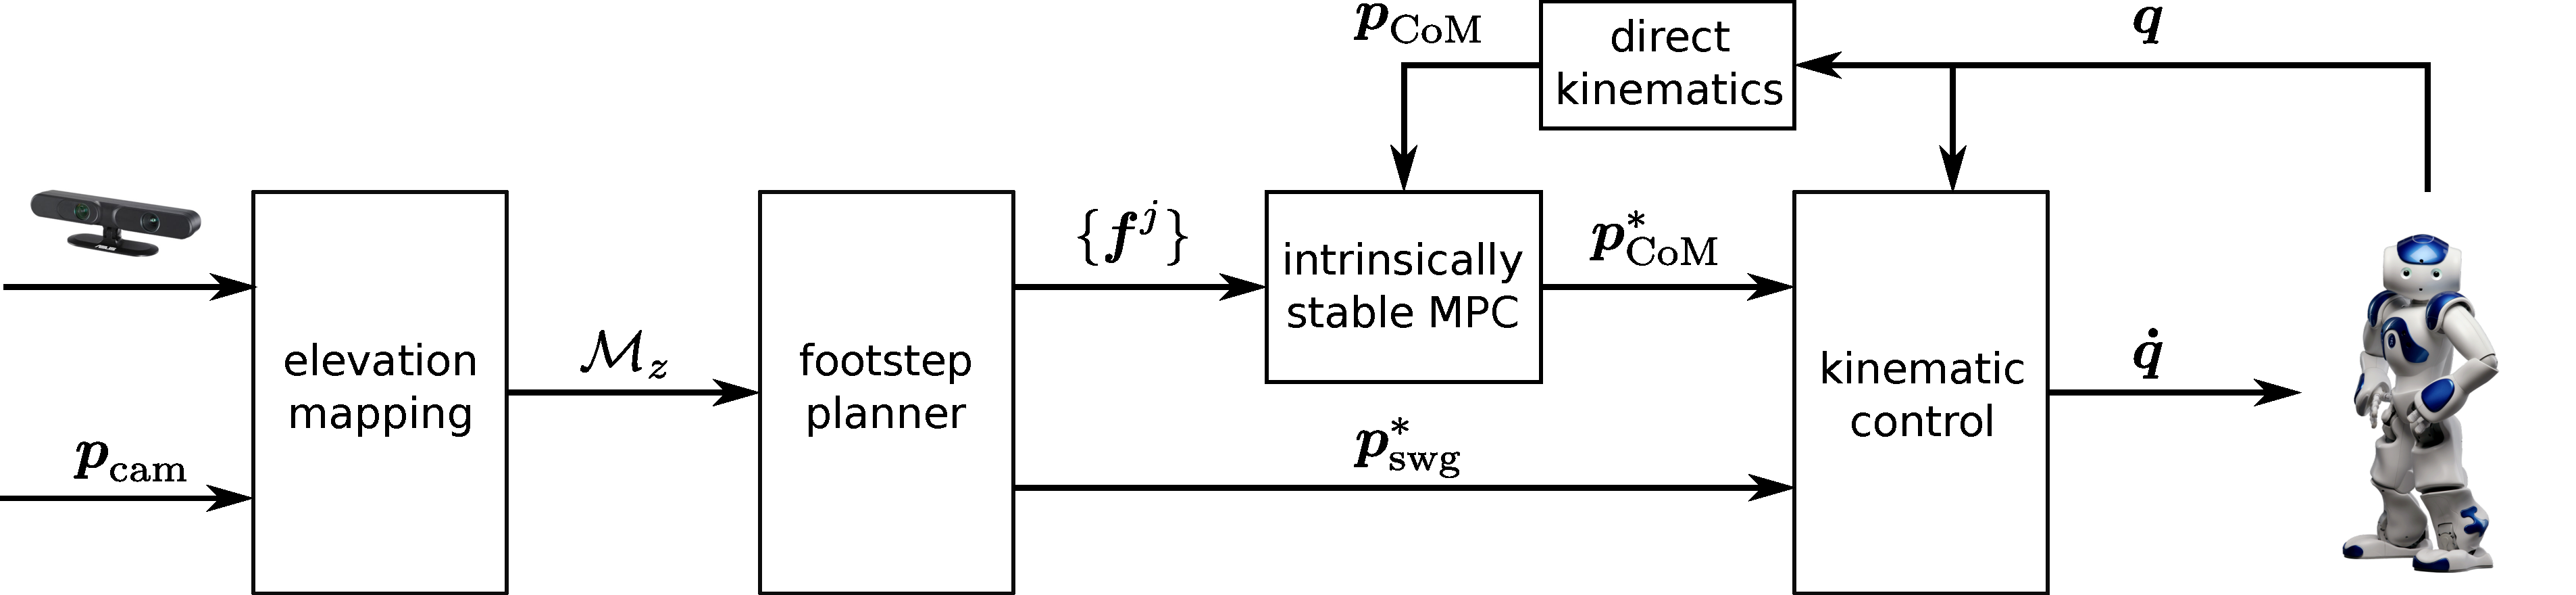
\includegraphics[width=\textwidth]{figures/BlockScheme.pdf}
  \caption{Block scheme of the approach.}
  \label{fig:block-scheme}
\end{figure}

\chapter{Elevation Map Generation}
\label{ch:elevation-map-generation}
When dealing with robot locomotion, the representation of the environment plays 
a fundamental role. It is, in fact, extremely important to properly
understand the structure of the world in order to safely make the robot move,
avoiding obstacles and dangerous zones, and to make it successfully complete 
its tasks. The world that surrounds the robot can be represented in many 
different ways; it is important to choose a proper representation to keep 
computational costs low and make to locomotion realizable.

In \textit{World of Stairs} scenarios, introduced in the previous chapter, the 
most efficient way to represent environments is by using elevation maps.
An elevation map is a grid that contains for each coordinate $(x, y)$ of the 
world its respective coordinate $z$. Hence, it can be seen as a function 
$\mathcal{M}_z$ such that, for each element $i$ of the grid,
$z_i = \mathcal{M}_z(x_i, y_i)$. This kind of representation allows the 
development of planners that quickly find plans to make robots move from a
position to another inside the world. 

This chapter introduces \texttt{elevation\_mapping}
\cite{Fankhauser2018ProbabilisticTerrainMapping}, the framework used in this 
thesis to generate elevation maps, which allow NAO to navigate in unknown 
environments (more precisely in \textit{World of Stairs} environments);
the ASUS Xtion Pro, an RGB-D sensor equipped on top of NAO, which has been 
used to send depth informaton to \texttt{elevation\_mapping}; 
the behaviour of the framework when a map is build using the ASUS Xtion Pro
placed on the head 
of NAO humanoid robot. The generated map is the one used in the experiment 
TODO and it is used by the footstep planner (Chapter
\ref{ch:rrt-based-footstep-planning}) to make NAO climb the stairs.

\section{Framework}
Todo (overview of elevation\_mapping). ROS.

\subsection{Definitions}
Todo (RFs).

\subsection{Map Update}
Todo (range measurements + robot motion).

\subsection{Map Fusion and Dynamic Environments}
Todo.

\section{ASUS Xtion Pro}
xtion (RGBD camera). ROS.
\begin{figure}
  \centering
  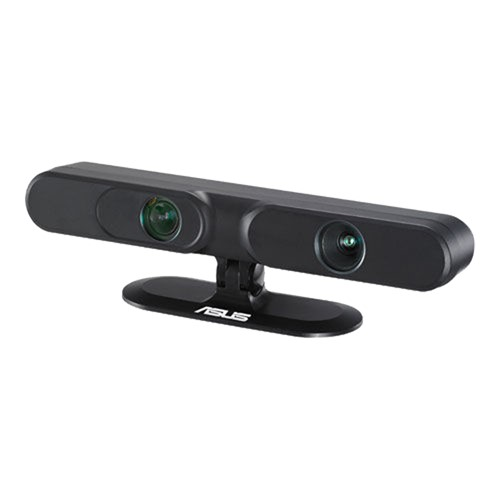
\includegraphics[width=0.5\textwidth]{figures/asus-xtion-pro.jpeg}
  \caption{The ASUS Xtion Pro is equipped with a depth sensor and it is 
      easily configurable to make it work with ROS. This simplifies the 
      integration with \texttt{elevation\_mapping} and, consequently, 
      the construction of a navigable map.}
  \label{fig:asus-xtion-pro}
\end{figure}

\section{World of Stairs}
(safe zone)
\begin{figure}
  \begin{subfigure}[b]{0.49\textwidth}
    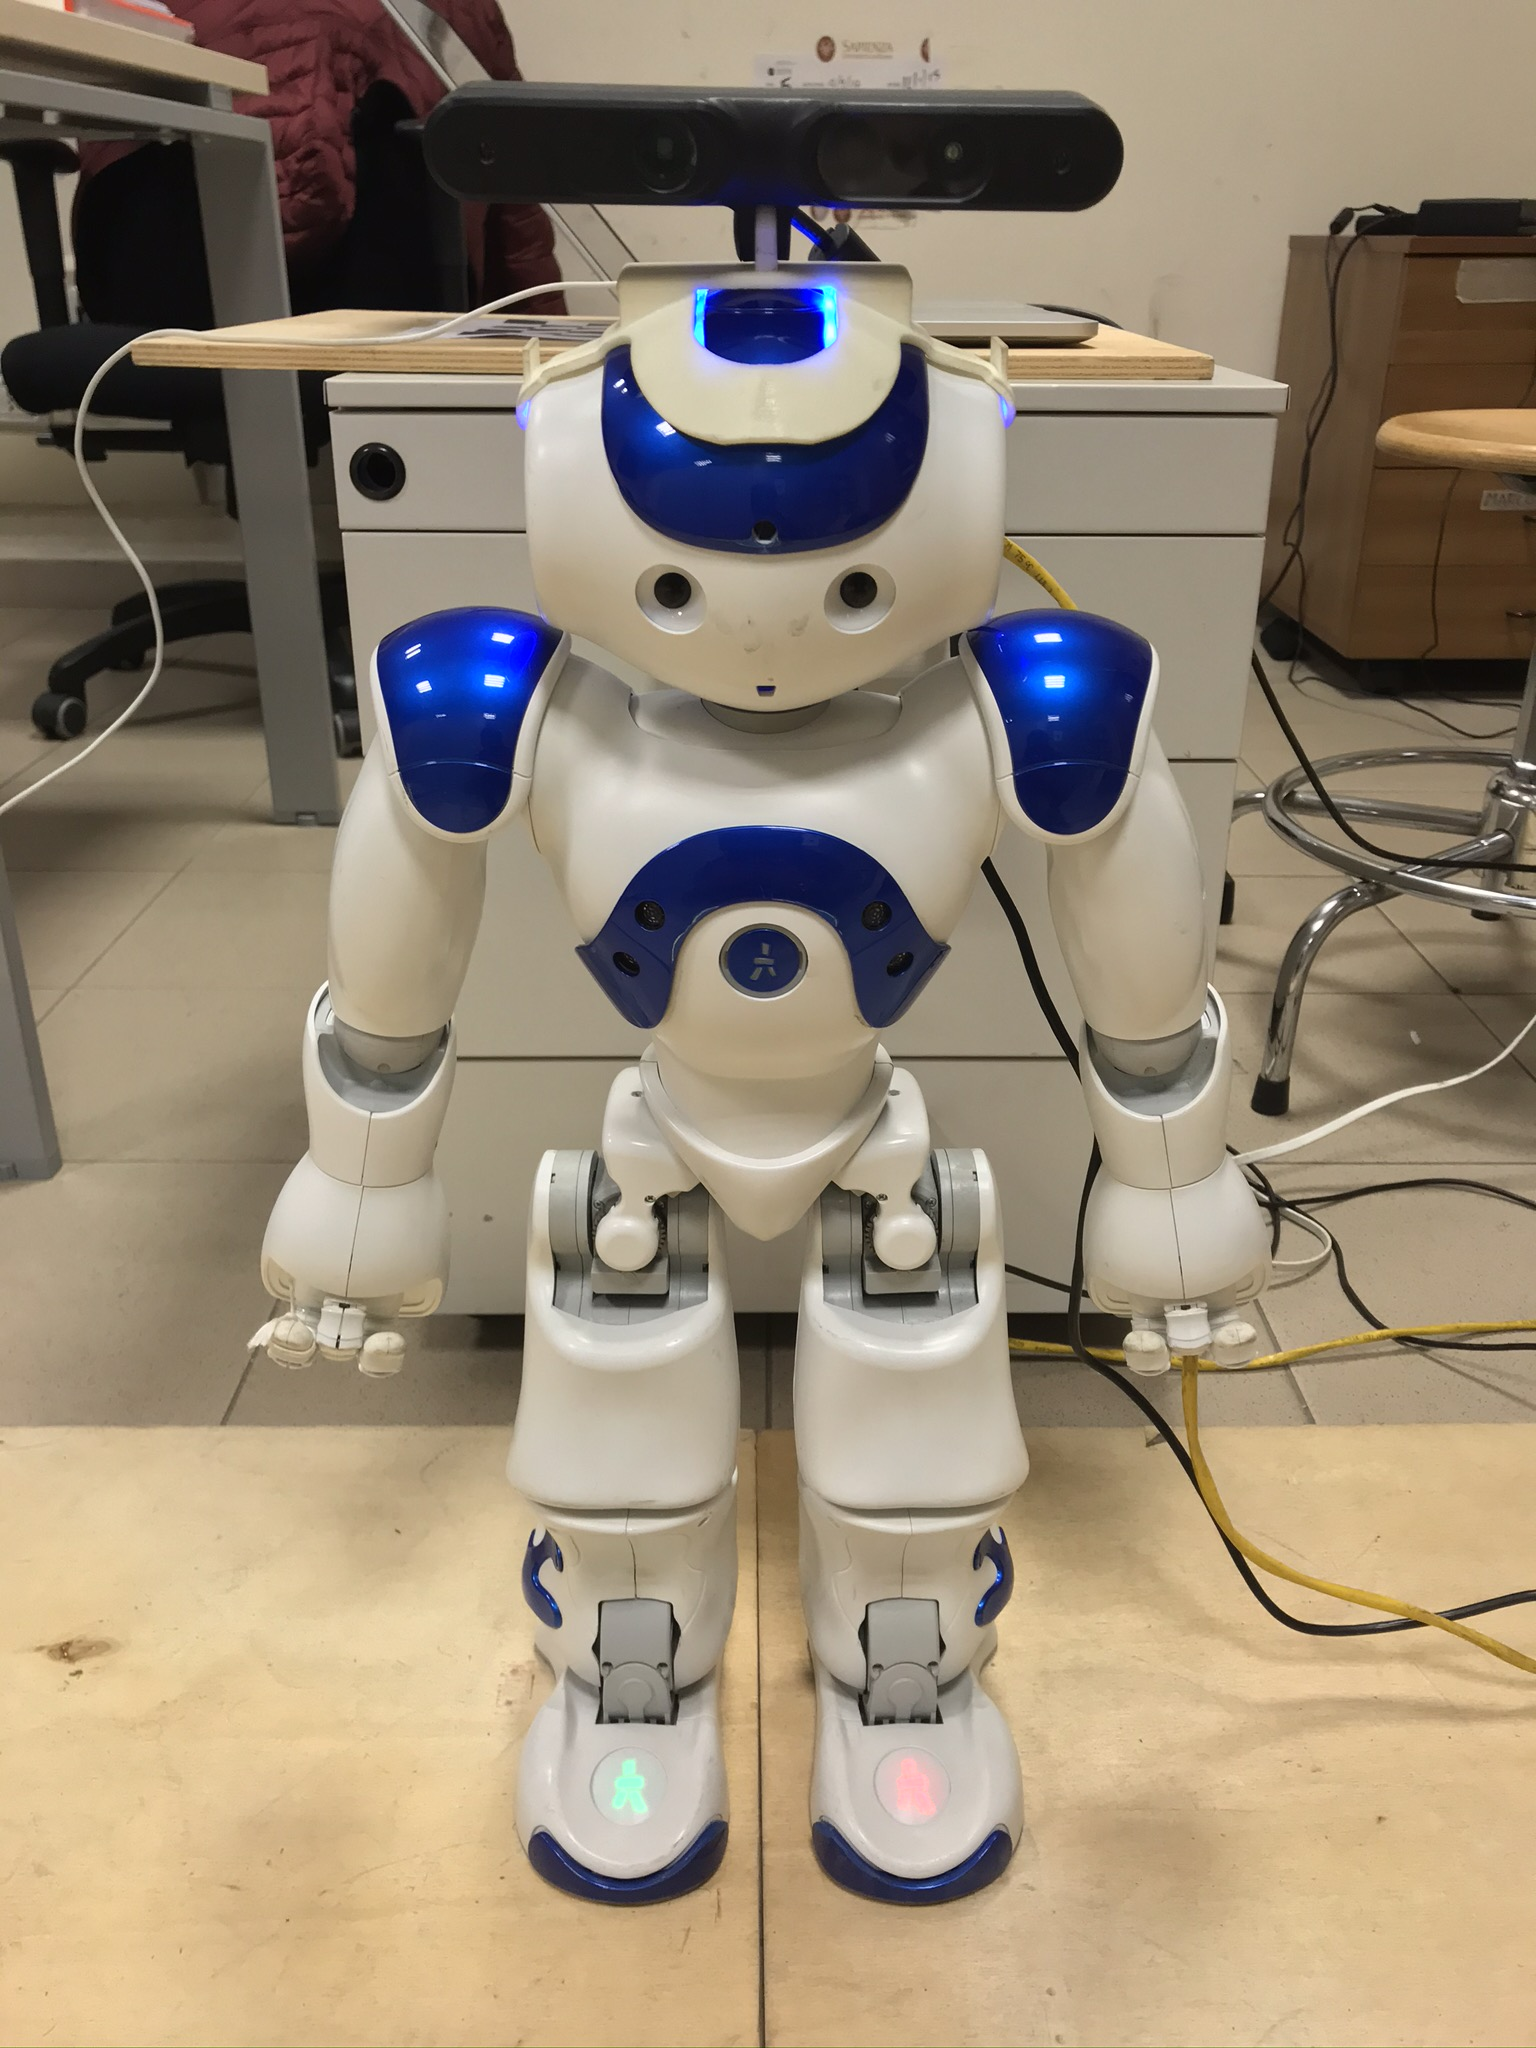
\includegraphics[width=\textwidth]{figures/NAO-with-xtion.JPEG}
    \caption{}
    \label{fig:nao-with-xtion}
  \end{subfigure}
  \hfill
  \begin{subfigure}[b]{0.49\textwidth}
    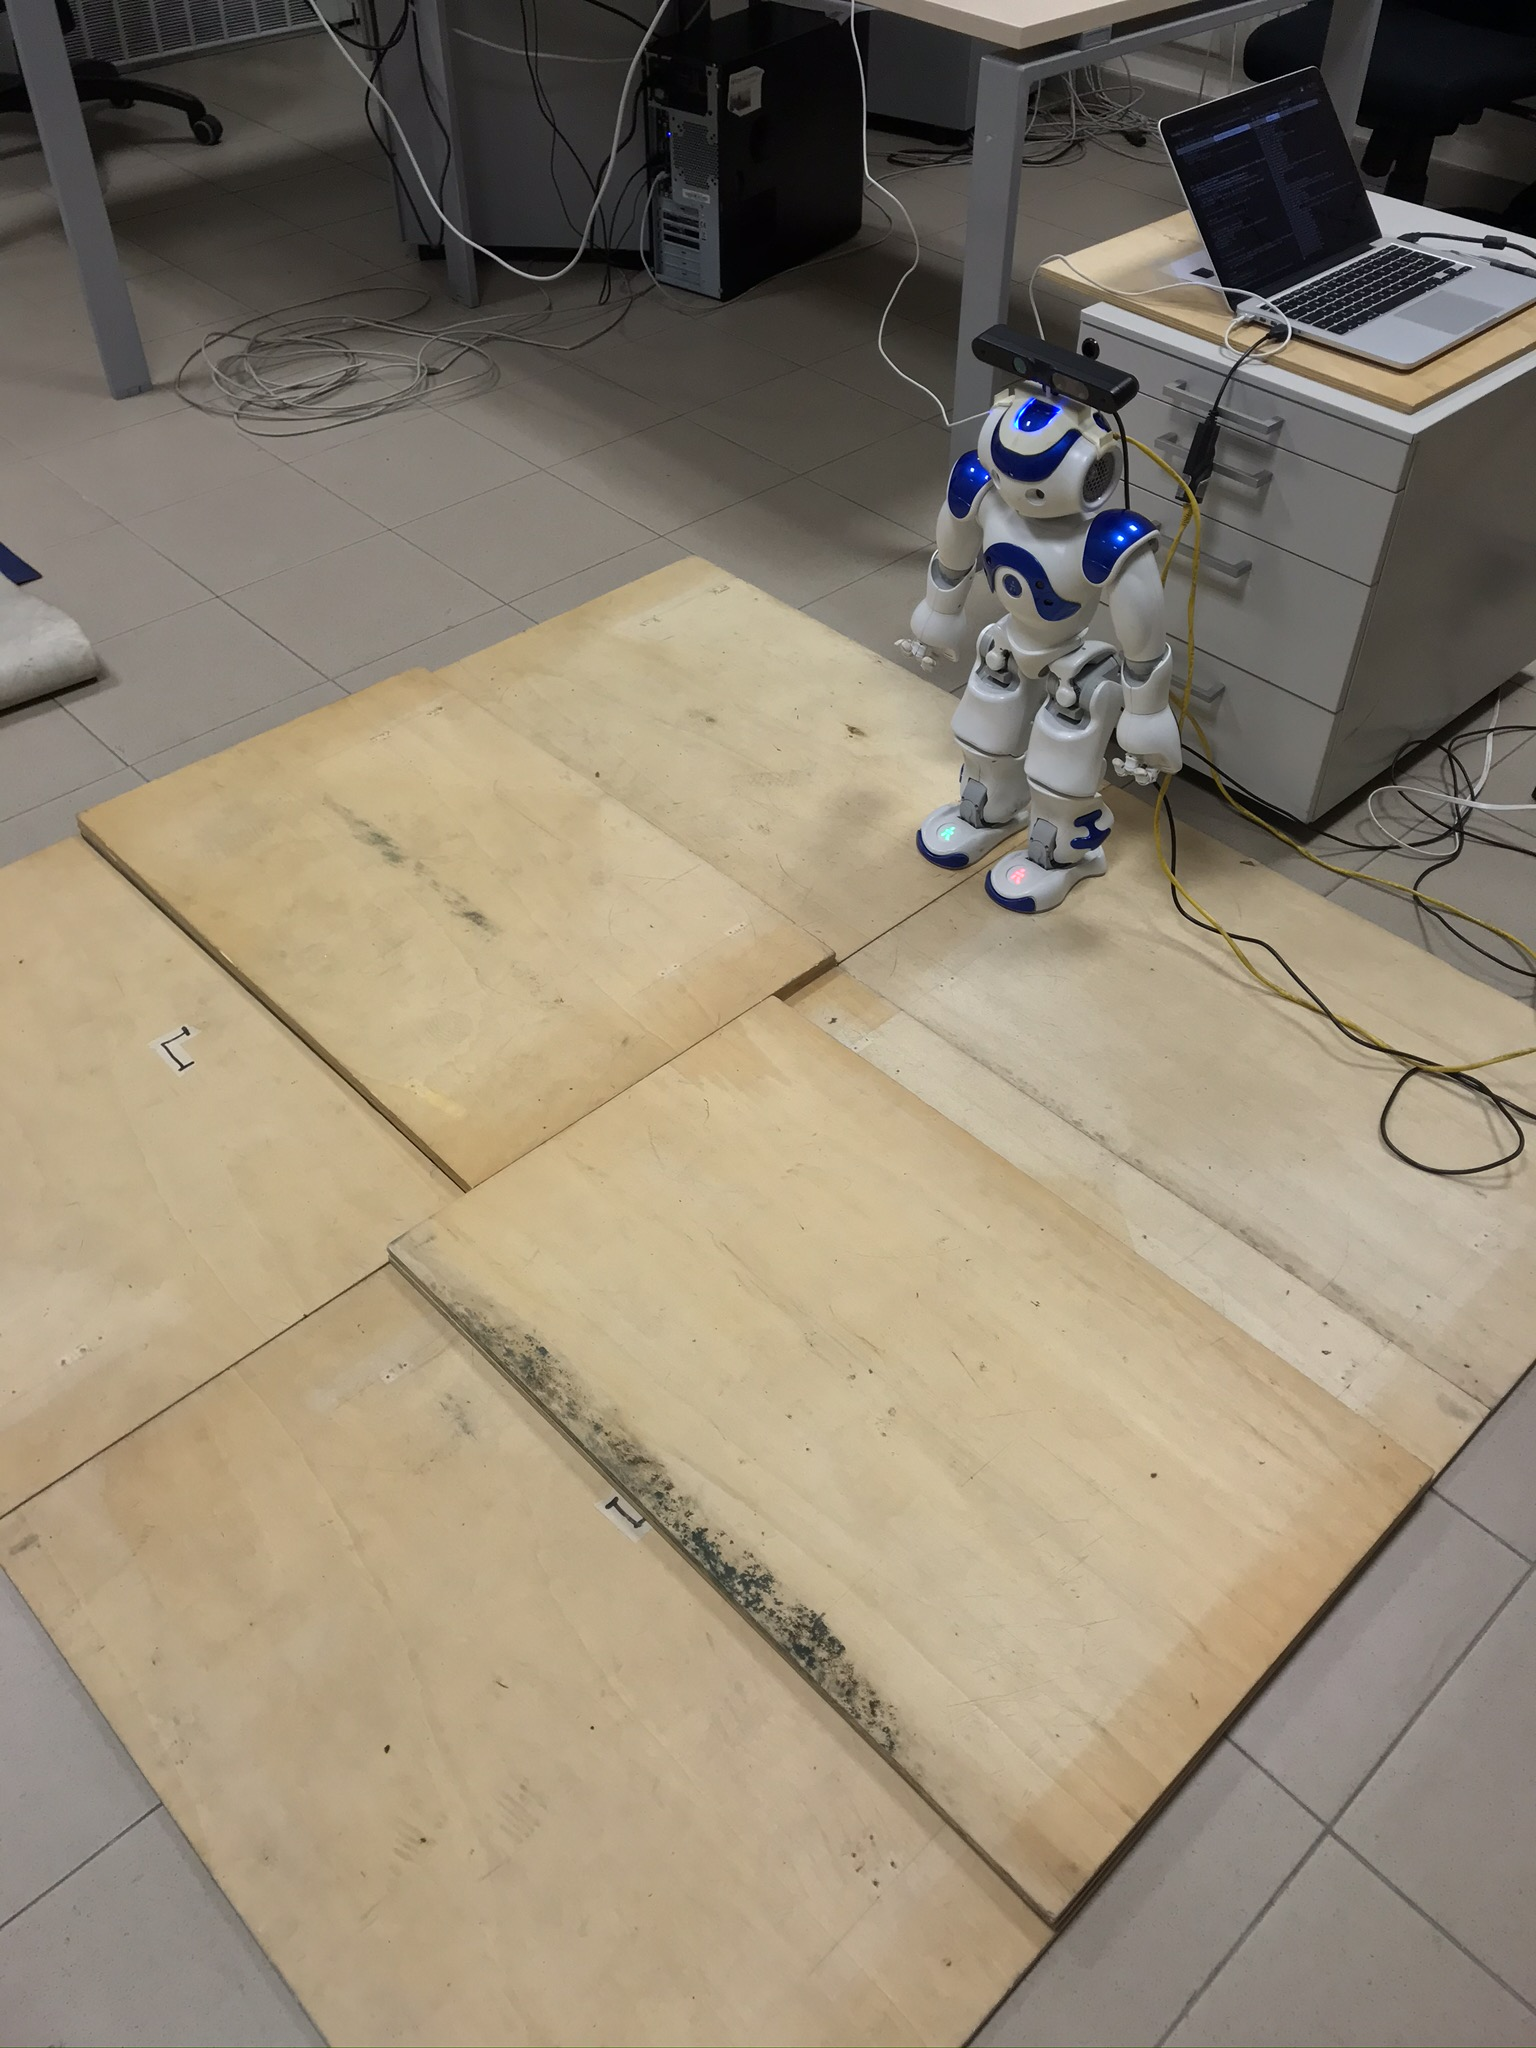
\includegraphics[width=\textwidth]{figures/NAO-with-xtion-full-env.JPEG}
    \caption{}
    \label{fig:nao-with-xtion-full-env}
  \end{subfigure}
  \caption{On the left, NAO humanoid robot with ASUS Xtion Pro placed on top.
      On the right, NAO humanoid robot in the environment described TODO, 
      right before starting the execution of the experiment.}
\end{figure}
\begin{figure}
  \centering
  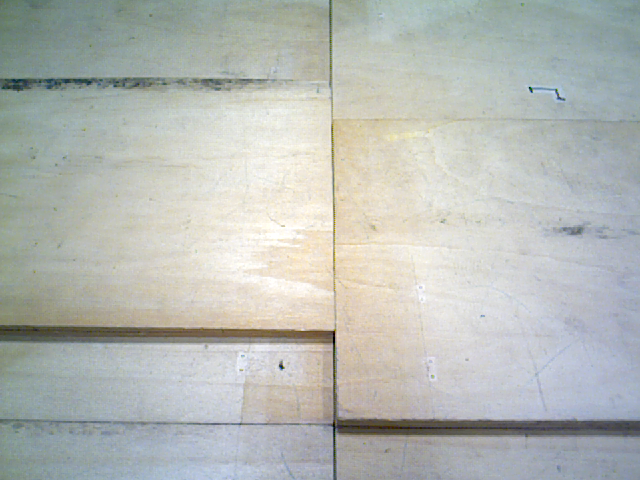
\includegraphics[width=0.85\textwidth]{figures/xtion_rgb_20cm.png}
  \caption{RGB image seen by the ASUS Xtion Pro placed on top of the robot.
      The corresponding depth image is sent to \texttt{elevation\_mapping}
      to build the map.}
  \label{fig:xtion-rgb-20cm}
\end{figure}
\begin{figure}
  \centering
  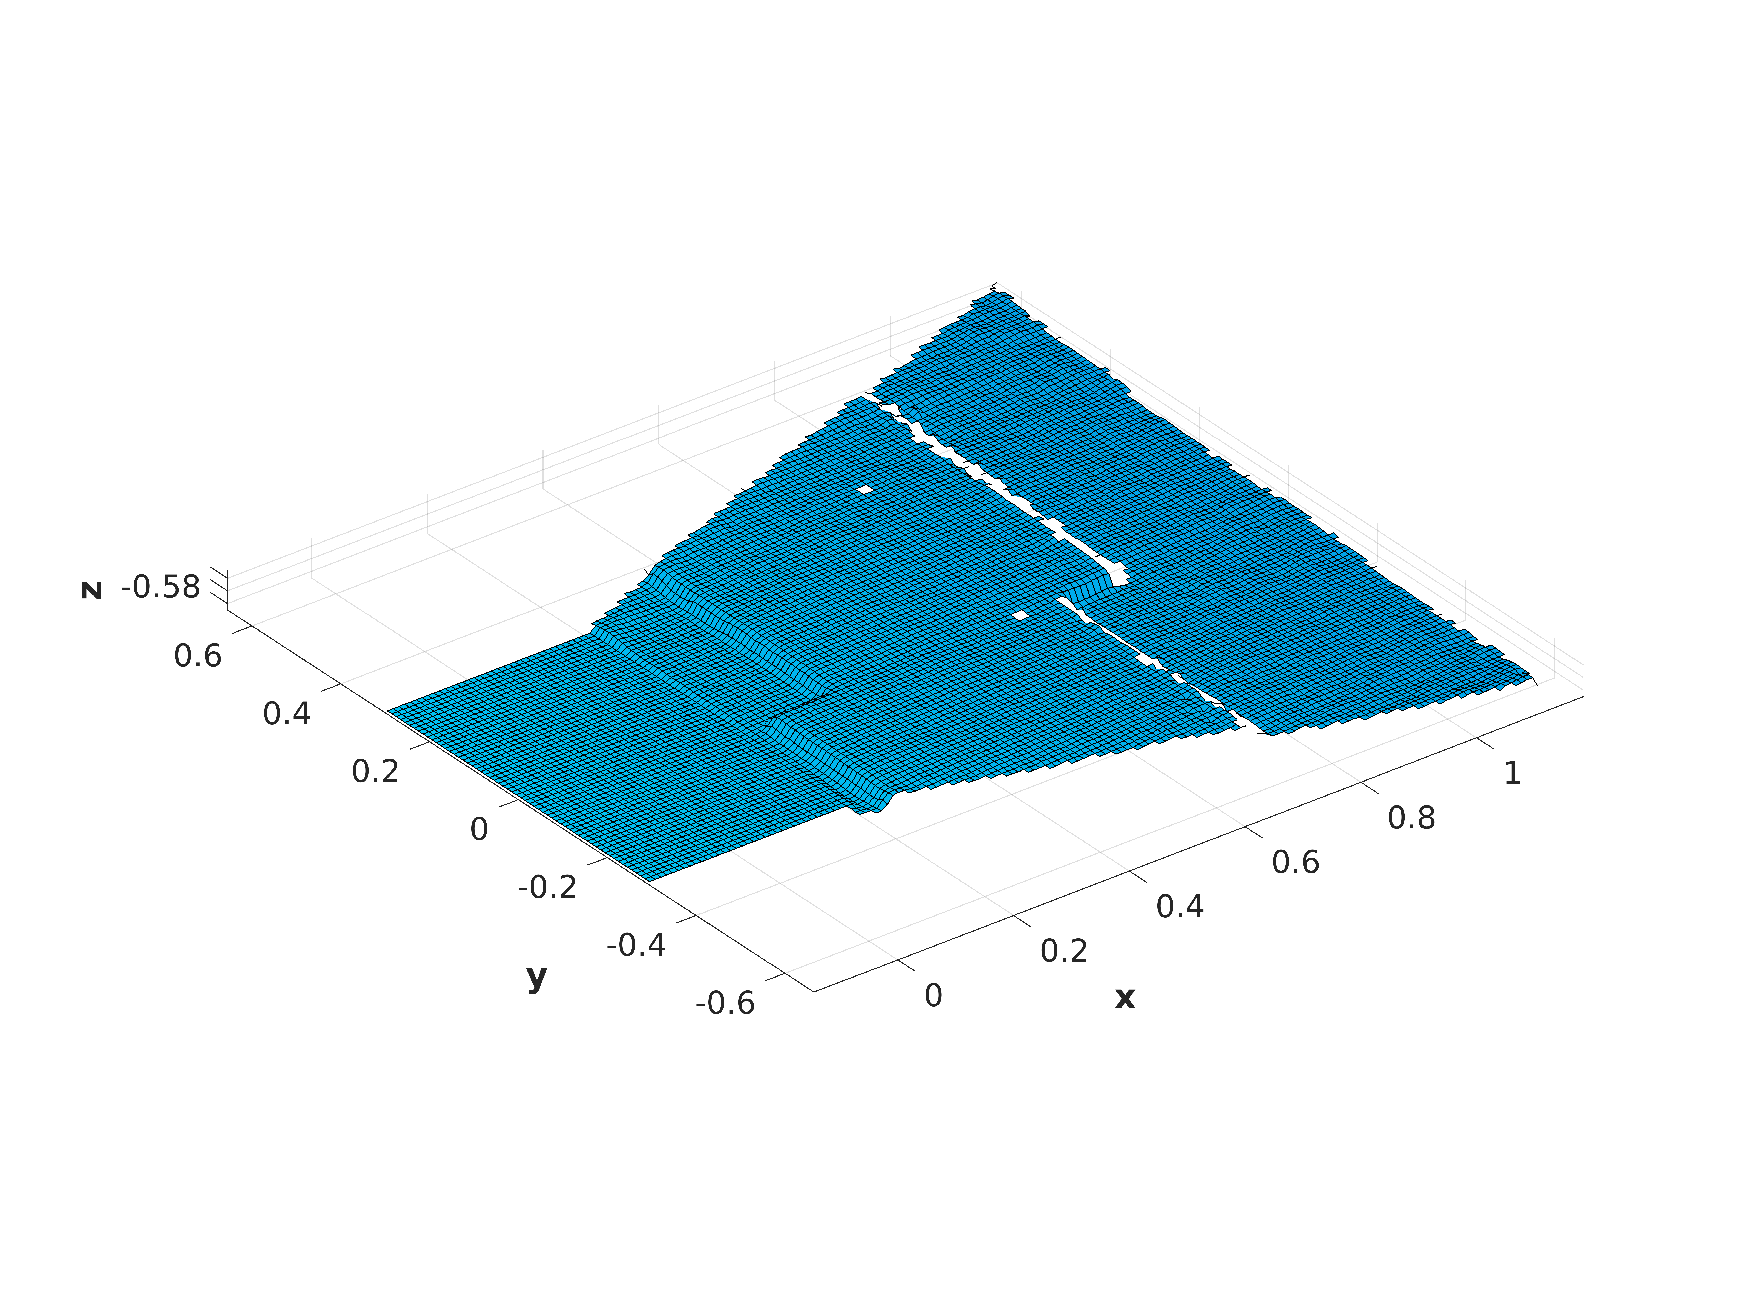
\includegraphics[width=\textwidth]{figures/onlymap-xtion-20cm.pdf}
  \caption{Elevation map build by \texttt{elevation\_mapping} for the scenario 
      ``Stair Climbing (Unknown Environment)'' described in section 
      \ref{sec:stair-climbing-unkenv}.}
  \label{fig:onlymap-xtion-20cm}
\end{figure}


\chapter{RRT-based Footstep Planning}
\label{ch:rrt-based-footstep-planning}

Considering the \textit{World of Stairs} scenarios discussed previously, the 
aim of a footstep planner is to determine a feasible sequence of footsteps that 
allows the humanoid robot to reach a desired goal region $\mathcal{G}$, given 
a representation of the environment, in this case the elevation map described in 
the previous chapter.

\section{Problem Formulation}
Before describing the algorithm, introduced in \cite{ECC19}, a more detailed 
formulation of the problem should be given.

\subsection{Notation and Plan Feasibility}
As introduced before, an 
elevation map is a proper choice for the representation of the scenarios 
described by \textit{World of Stairs}, since it is efficient to store and to 
query. Let's denote the map by $\mathcal{M}_z$. The height from the ground of
a cell having coordinate $(x, y)$ is $z = \mathcal{M}_z(x, y)$.

Given $\mathcal{M}_z$, the goal of the footstep planner (offline) is to find 
a feasible sequence of footsteps $\{\bff^j\}$ which leads to a desired location 
$\mathcal{G}$, together with the corresponding swing foot trajectories
$\{\bfp_{\rm {swg}}^j\}$. Let's denote $\bff^j = (x_{\rm f}^j, y_{\rm f}^j,
z_{\rm f}^j, \theta_{\rm f}^j)^T$ as the pose of the $j$-th footstep, 
with $x_{\rm f}^j, y_{\rm f}^j, z_{\rm f}^j$ position of the footstep and 
$\theta_{\rm f}^j$ yaw orientation of the footstep. Note that in the scenarios 
represented by \textit{World of Stairs} the roll and pitch angles of the 
footsteps are always zero.

In order to make the footstep plan feasible, let's introduce the following 
requirements:
\begin{itemize}
  \item[R1] The height variation between two consecutive footsteps is with 
      a maximum range: $|z_{\rm f}^j - z_{\rm f}^{j-1}| \le \Delta z_{\max}$.
  \item[R2] The footstep is fully in contact within the ground, hence,
      each cell of $\mathcal{M}_z$ which belongs to the footprint has the 
      same height $z_{\rm f}^j$.
  \item[R3] The swing foot trajectory $\bfp_{\rm {swg}}^j$ is collision free
      (apart of course at the start and at the end of the trajectory itself).
\end{itemize}

Once the footsteps have been generated, they are passed to an online gait 
generation block (described in Chapter \ref{ch:vh-com-is-mpc}) which computes
the 
optimal CoM trajectory $\bfp_{\rm CoM}^*$ that allows the humanoid robot to
execute the plan. The optimal swing foot trajectory $\bfp_{\rm {swg}}^*$ is 
defined by the appropriate subtrajectory $\bfp_{\rm {swg}}^j$.

The reference trajectories $\bfp_{\rm {swg}}^*, \bfp_{\rm {swg}}^j$ are passed
to a pseudoinverse-based kinematic controller to compute joint commands
$\dot{\bfq}$ for the robot.
Proprioceptive feedback is used for both gait generator block 
and kinematic controller.

\section{Algorithm}
The following algorithm \cite{ECC19}, which is based on RRT (Rapidly Exploring
Random Tree), finds a feasible sequence of footsteps in a
\textit{World of Stairs} scenario given the elevation map $\mathcal{M}_z$ of the 
environment,
the goal region $\mathcal{G}$ and the starting configuration of the feet
$\bff_L, \bff_R$. The generated sequence connects the starting point to the
goal.

\subsection{Pseudocode}
The footstep planner, whose behaviour is described by Algorithm
\ref{alg:footstep-planner} iteratively builds a tree $\mathcal{T}$ of feet 
configurations in a randomized way. In general, a vertex $v=(\bff_{\rm {sup}},
\bff_{\rm {swg}})$ specifies the pose of the support foot and the swing foot 
during the phase of double support. An edge connecting two vertices exists 
when there exists a collision free trajectory of the swing foot between 
the two configurations.

The algorithm starts by initializing the tree with the initial configuration of 
the left and the right foot (line 1). At each iteration, a point 
$\bfp_{\rm {rand}}$ is selected randomly on the ground (line 5). Here, the 
planner randomly choose between exploration and exploitation mode. In the first 
case $\bfp_{\rm {rand}}$ is generated by randomly selecting a pair of 
coordinates $x, y$ and retrieving the $z$ corrdinate from the elevation map 
$\mathcal{M}_z$. In the second case $\bfp_{\rm {rand}}$ is sampled from
$\mathcal{G}$. At this point, the vertex $v_{\rm {near}}$ of $\mathcal{T}$
that is closest to $\bfp_{\rm {rand}}$ is selected (line 6) in order to check
whether it can be connected to the tree $\mathcal{T}$. The distance between
$v_{\rm {near}}$ and $\bfp_{\rm {rand}}$ is determined using the following
metric:
\begin{equation}
  \gamma(v, \bfp) = d(\bfm, \bfp) + \alpha |\theta_p|
\end{equation}
where $d(\bfm, \bfp)$ is the Euclidean distance between the midpoint $\bfm$
between the feet (hence, between $\bff_{\rm {sup}}$ and $\bff_{\rm {swg}}$ in
$v$) and $\bfp$, $\theta_p$ is the angle between the robot sagittal axis and 
the line joining $\bfm$ to $\bfp$, and $\alpha>0$. Once $v_{\rm near}$ has been 
selected, the foot poses $\bff_{\rm sup}^{\rm near}, 
\bff_{\rm {swg}}^{\rm near}$ are extracted from it. A candidate footstep
$\bff^{\rm cand}$ is randomly generated (line 7) by selecting a final pose of
the swing foot from the catalogue of primitives U defined with respect to 
$\bff_{\rm sup}^{\rm near}$, as shown in Fig. \ref{fig:catalogue-primitives} and 
defined in the next section. As before, the $z$ coordinate of $\bff^{\rm cand}$
is determined by $\mathcal{M}_z$. On line 8, requirements R1-R2 defined above 
are checked for $\bff^{\rm cand}$. In positive case, a collision checking 
algorithm (lines 9-13) is performed to verify whether there exists a collision 
free trajectory $\bfp_{\rm swg}^{\rm cand}$ (a second degree polynomial
equation)
that brings the swing foot from 
$\bff_{\rm swg}^{\rm near}$ to $\bff^{\rm cand}$. In positive case, also 
requirement R3 is verified and a new vertex $v_{\rm new} = (\bff^{\rm cand}, 
\bff_{\rm \sup}^{\rm near})$ is added to the tree $\mathcal{T}$ as a child of 
$v_{\rm near}$ (lines 14-17). The algorithm terminates when the midpoint 
$\bfm$ between the feet at the new vertex $v_{\rm new}$ is inside the goal 
region $\mathcal{G}$ or a maximum number of iterations $i_{\max}$ has been 
reached (line 18). When a solution has been found, the path joining the 
initial vertex $(\bff_L, \bff_R)$ to $v_{\rm new}$ is extracted from the tree 
and the footstep sequence $\{\bff^j\}$ is reconstructed together with the 
swing foot trajectories $\{\bfp_{\rm swg}^j\}$.

\begin{algorithm}
%  \small
%  \removelatexerror
  \caption{Footstep Planner}
  \label{alg:footstep-planner}
  root the tree $\mathcal{T}$ at $v_{\rm ini} \leftarrow (\bff_L, \bff_R)$\;
  $i \leftarrow 0$\;
  \Repeat{$\bfm \in \cal G$ \rm{\textbf{or}} $i = i_{max}$}{
    $i \leftarrow i+1$\;
    generate a random point $\bfp_{\rm rand}$ on the ground\;
    select the closest vertex $v_{\rm near}$ in $\cal T$ to $\bfp_{\rm rand}$
        according to $\gamma(\cdot, \bfp_{\rm 	rand})$\;
    randomly select from the primitive catalogue $U$ a candidate footstep
        $\bff^{\rm cand}$\;
    \If{$\bff^{\rm cand}$ {\rm is feasible w.r.t.\ R1--R2}}{
      $h \leftarrow h_{\rm min}$\;
      $\bfp^{\rm cand}_{\rm swg} \leftarrow$
          BuildTrajectory$(\bff_{\rm swg}^{\rm near}, \bff^{\rm cand}, h)$\;					
      \While{$h \leq h_{\rm max}$ \rm{\textbf{and}}
          \rm Collision($\bfp_{\rm swg}^{\rm cand}$)}{
        $h \leftarrow h + \Delta h$\;
        $\bfp^{\rm cand}_{\rm swg} \leftarrow$
            BuildTrajectory$(\bff_{\rm swg}^{\rm near}, \bff^{\rm cand}, h)$\;		
      }
      \If{$h \leq h_{\rm max}$}{
        $v_{\rm new} \leftarrow (\bff^{\rm cand},\bff_{\rm sup}^{\rm near})$\;	
        add vertex $v_{\rm new}$ to $\cal T$ as a child of $v_{\rm near}$\;
        compute midpoint $\bfm$ between the feet at $v_{\rm new}$\; 
      }				
    }	
  }	
\end{algorithm}

\section{Implementation}
The planner has been implemented in C++ and it has been tested on both dynamic 
environments and NAO humanoid robot. The elevation map is either
generated by the 
\texttt{elevation\_mapping} framwork or manually generated before the execution 
of the program. Experiments are described in detail in Chapter 5. Note that to 
simplify the communication between \texttt{elevation\_mapping} and the planner 
and the communication between the planner and the robot, the planner has been 
executed on an external computer, which is connected to the robot through 
an ethernet cable. The plan is sent through TCP. The communication is designed 
with the idea to extend the planner in order to handle replanning phases and
dynamic environments.
\ref{ch:experiments} 
\subsection{Catalogue of Primitives}
As mentioned before, the catalogue of primitives specifies the possible 
footsteps that the robot can perform at each step. In this thesis the catalogue 
for the NAO humanoid robot (left foot with respect to right foot)
has been defined as:
\begin{equation}
  (x, y, \theta) \in \{ -6.0, 0.0, 6.0, 8.0, 10.0 \} \times
      \{ 11.0, 12.0 \} \times \{ 0, \pi/12 \}
\end{equation}
The catalogue of primitives of the right foot with respect the left foot is 
symmetric and it is shown in Fig. \ref{fig:catalogue-primitives}.
\begin{figure}
    \centering
    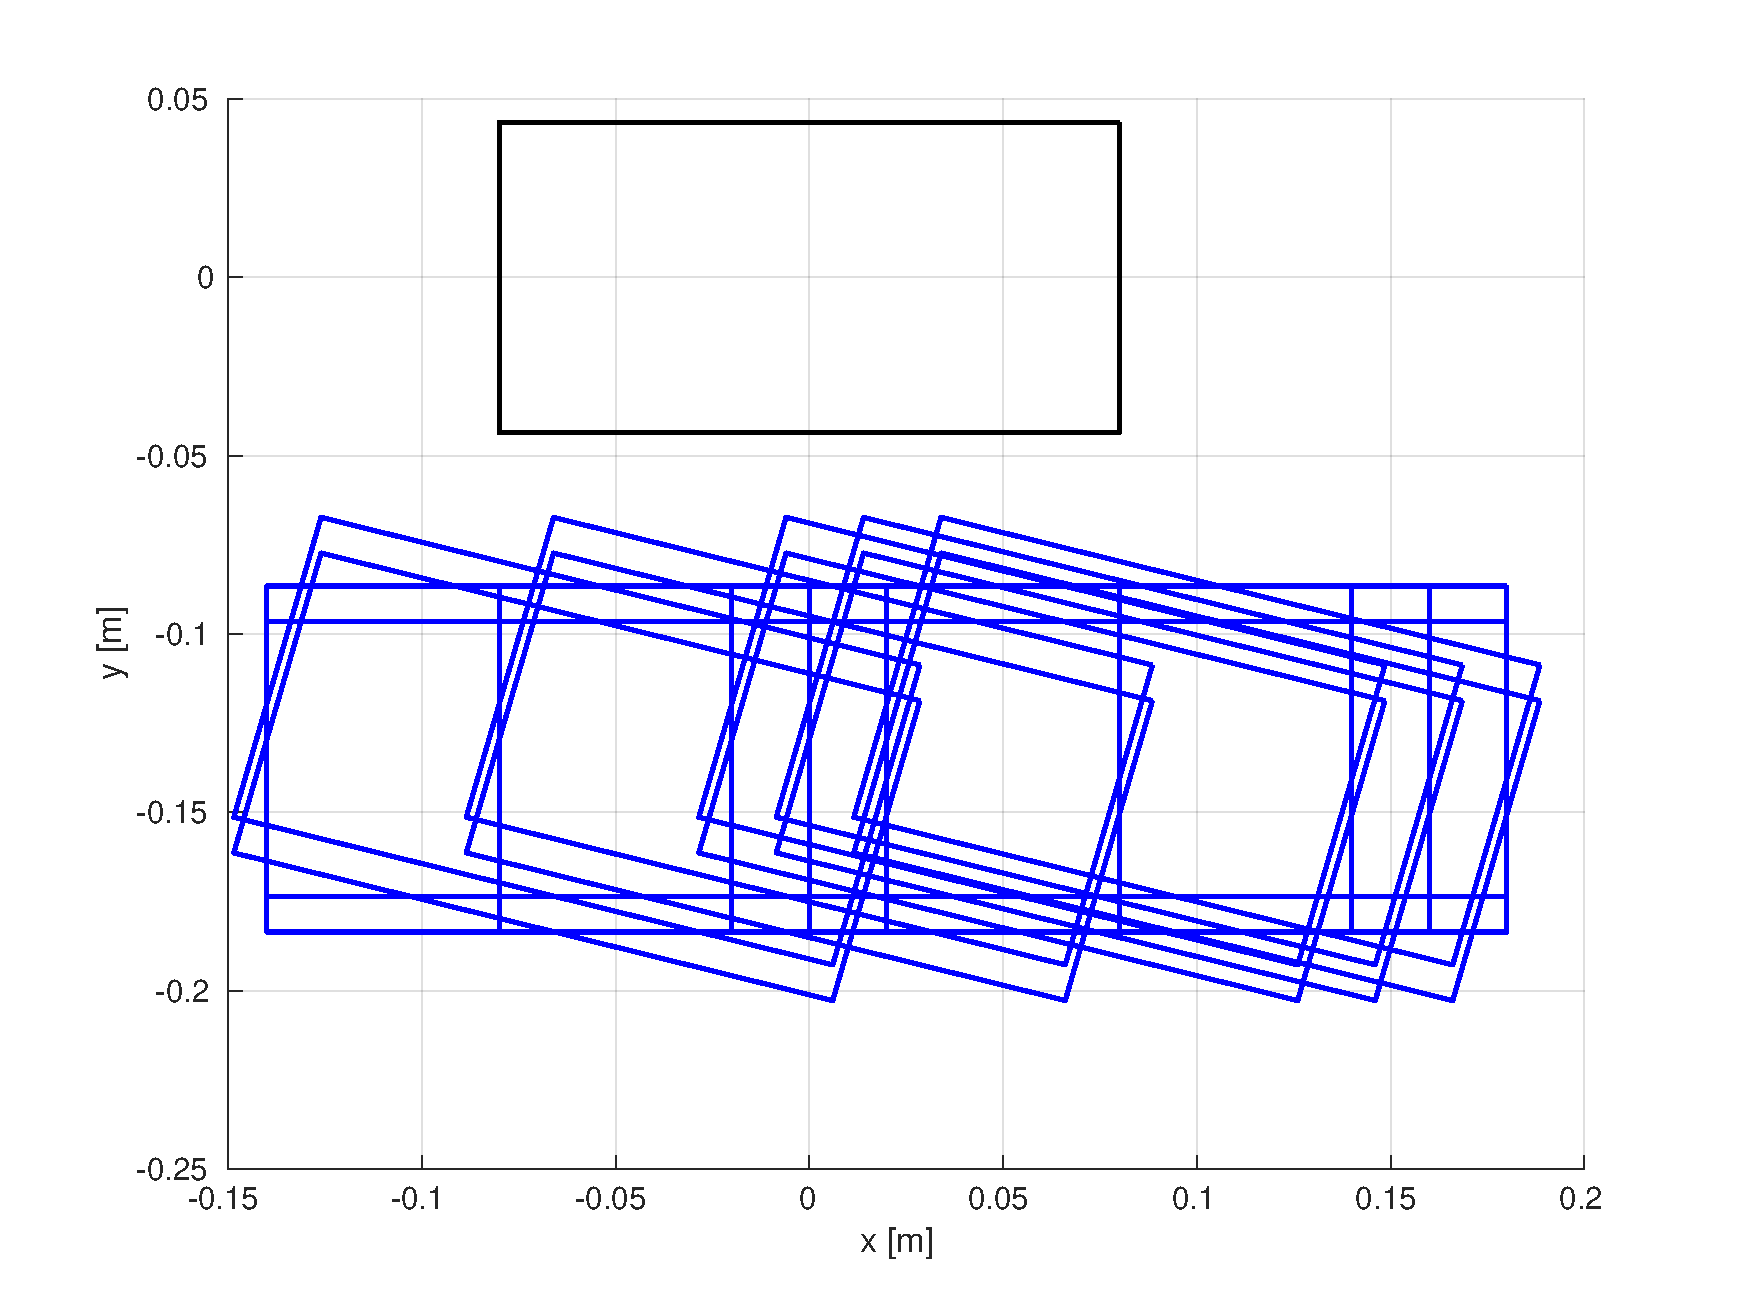
\includegraphics[width=\textwidth]{figures/catalogue-primitives.pdf}
    \caption{The catalogue of primitives (blue color) specifies the possible
        poses of the
        candidate footstep $\bff^{\rm cand}$ with respect to the pose of the 
        current support foot $\bff_{\rm sup}^{\rm near}$. The figure shows the 
        case where the left foot is the support foot. The catalogue for the 
        case where the right foot is the support foot is specular. The $z$
        coordinate of a candidate footstep can be retrieved directly from 
        the elevation map $\mathcal{M}_z$.}
    \label{fig:catalogue-primitives}
\end{figure}
The footstep planning hyperparameters have been set in the following way:
the goal region has been defined as a circle of radius $0.01 {\rm m}$,
$\alpha=1$,
$\Delta z_{max}=0.045 {\rm m}$, $h_{\min}=0.02 {\rm m}$,
$h_{\max}=0.07 {\rm m}$, $\Delta h=0.01 {\rm m}$.
The resolution of $\mathcal{M}_z$ has been set to $0.01 {\rm m}$ when using maps 
generated by \texttt{elevation\_mapping} and to $0.02 {\rm m}$ when using maps 
generated manually.


\chapter{Variable Height CoM IS-MPC}
\label{ch:vh-com-is-mpc}
Before describing in detail the model \cite{SYROCO18} that allows humanoid 
robots to walk on uneven terrain (in this case \textit{World of Stairs}),
it is important to introduce the notation and 
to make an overview of the previous works.
Differently from manipulators, which are fixed to the ground, humanoids need 
to maintain equilibrium while walking. The contact with the ground is, in fact,
continuously changed due to walking itself. Usually, this is achieved by 
making sure that the ZMP (Zero Moment Point) is always within the convex hull 
of the support polygon. The ZMP, introduced in \cite{VUKOBRATOVIC19721}, is the 
point where the horizontal component of the moment of the ground reaction forces
becomes zero. To generate this kind of motion, usually a simplified model 
which only considers the CoM (center of mass) of the robot is used.
In particular, by neglecting the robot angular momentum and by assuming the 
CoM height is constant, the CoM dynamics can be treated as a LIP (Linear 
Inverted Pendulum), introduced for the first time in \cite{Kajita1991StudyOD}.
The Linear Inverted Pendulum model easily allows to design control schemes for 
the generation of the CoM reference trajectory, like the Preview Control 
\cite{Kajita2003BipedWP} and the Model Predictive Control
\cite{wieber:inria-00390462}.
Before discussing the LIP and extending it to the Variable Length Inverted
Pendulum, let's discuss the 3D motion model of the CoM reminding that the CoP
(Center of Pressure) in case of flat ground is the point of application of
the ground reaction force.

\section{3D Motion Model}
Let $(x_z, y_z, z_z)$ and $(x_c, y_c, z_c)$ respectively be the position of 
the ZMP and the position of the CoM. Assuming that the humanoid robot is walking 
on flat ground (hence the gravity acceleration components on $x$ and $y$ are 
zero) and neglecting the angular momentum around the CoM, the ZMP can be 
anywhere along the line connecting the CoP (located on the piece of surface 
upon which the support foot is placed) and the CoM (Fig. \ref{fig:lipm-robot}),
it is possible
\cite{kajita:intro-humanoid-robotics} to obtain the dynamics of the CoM:
\begin{align}
  \ddot{x}_c &= \frac{\ddot{z}_c + g}{z_c - z_z} (x_c - x_z) \\
  \ddot{y}_c &= \frac{\ddot{z}_c + g}{z_c - z_z} (y_c - y_z) \\
  \ddot{z}_c &= \frac{f_z}{m} - g
\end{align}
where $g$ is the gravity acceleration, $f_z$ is the z-component of the ground
reaction force, acting as an external input, and $m$ is the total mass of
the humanoid robot.
\begin{figure}
    \centering
    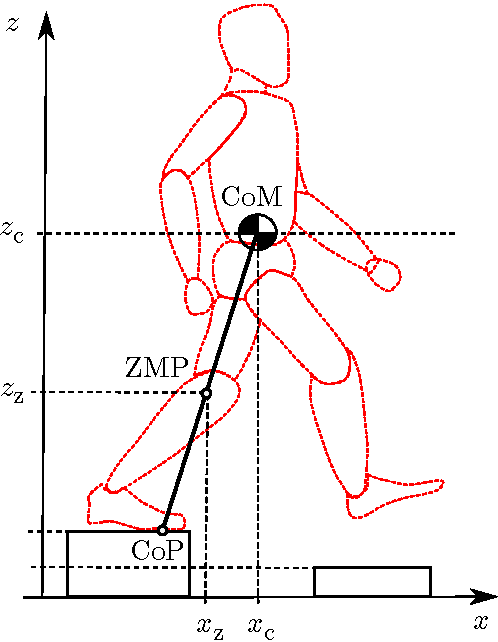
\includegraphics[width=0.5\textwidth]{figures/LIPM_robot.pdf}
    \caption{When walking on flat ground, or more in general on
        piecewise-horizontal ground as in the figure, the ZMP can be anywhere 
        between the line connecting the CoP and the CoM.}
    \label{fig:lipm-robot}
\end{figure}
The condition for maintaining equilibrium is that CoP is internal to the 
support polygon. Since the CoP, the CoM and the ZMP are colinear, as shown in 
Fig. \ref{fig:balance3d}, the condition is equivalent to the ZMP being internal
to the polyhedral cone having CoM as vertex and support
polygon as cross-section.
\begin{figure}
    \centering
    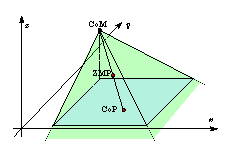
\includegraphics[width=0.7\textwidth]{figures/balance3d.pdf}
    \caption{The CoP should be internal to the support polygon, which is 
        equivalent to the ZMP being internal to the polyhedral cone with 
        the CoM as a vertex.}
    \label{fig:balance3d}
\end{figure}

\section{LIP}
The above motion model is nonlinear and difficult to use for gait generation.
Usually, to make the model linear, it is assumed that the ground is horizontal 
and the CoM has constant elevation with respect to the ground (i.e.
$z_c=\bar{z_c}$). As a consequence, it is possible to set $z_z=0$ making the 
CoP and the ZMP coincident, hence obtaining the LIP model:
\begin{align}
  \ddot{x}_c &= \omega_0^2 (x_c - x_z) \label{eq:lipm-x} \\
  \ddot{y}_c &= \omega_0^2 (y_c - y_z) \label{eq:lipm-y}
\end{align}
where $\omega_0^2 = g/\bar{z}_c$. This linear model, however, is not suitable 
for gait generation over uneven terrain.

\section{Variable Height CoM Motion Model}
Requiring the CoM to move at a constant height is not the only way to make the 
system linear. A more general way is to constraint its vertical motion such
that:
\begin{equation}
  \frac{\ddot{z}_c + g}{z_c - z_z} = \omega^2
\end{equation}
with $\omega$ arbitrary constant.

Using the above equation, the CoM dynamics become:
\begin{align}
  \ddot{x}_c &= \omega^2 (x_c - x_z) \label{eq:com-dynamics-x} \\
  \ddot{y}_c &= \omega^2 (y_c - y_z) \label{eq:com-dynamics-y}\\
  \ddot{z}_c &= \omega^2 (z_c - z_z) - g \label{eq:com-dynamics-z}
\end{align}
The above equations are linear and have a LIP-like structure with the 
ZMP coordinates $(x_z, y_z, z_z)$ acting as control inputs. This 3D model,
against the model of the LIP described in Eqs.
(\ref{eq:lipm-x}-\ref{eq:lipm-y}), allows vertical motion of the CoM, thus,
it can be used for 
gait generation on uneven terrain, considering the balance condition 
described by Fig. \ref{fig:balance3d}.

\section{MPC Formulation}
Before describing an MPC scheme for gait generation based on the above 
equations, it is important to notice that all of them include an unstable 
subsystem. For example, let's consider Eq. \eqref{eq:com-dynamics-x}. It is 
possible to decompose the system into a stable and an unstable subsystem by 
performing the following change of coordinates:
\begin{align}
  x_s = x_c - \dot{x}_c / \omega \\
  x_u = x_c + \dot{x}_c / \omega
\end{align}
The dynamics of $x_u$ is:
\begin{equation}
  \dot{x}_u = \dot{x}_c + \omega (x_c - x_z)
\end{equation}
which is unstable. It is however possible to prove 
\cite{Lanari2014BoundednessII} that $x_u$, and consequently $x_c$, will not 
diverge if a certain initial condition is satisfied (discussed in section 
\ref{sec:mpc-stability-constraint}). The same 
reasoning applies for the other two variables.

Let's perform a dynamic extension and choose the control variable as the ZMP 
velocities $\dot{x}_z, \dot{y}_z, \dot{z}_z$ rather than the ZMP itself. On the 
$x$ axis, the motion model becomes:
\begin{equation}
  \label{eq:vhcomlip-motion-model}
  \begin{pmatrix}
    \dot{x}_c \\
    \ddot{x}_c \\
    \dot{x}_z
  \end{pmatrix}
  =
  \begin{pmatrix}
    0 & 1 & 0 \\
    \omega^2 & 0 & -\omega^2 \\
    0 & 0 & 0
  \end{pmatrix}
  \begin{pmatrix}
    x_c \\
    \dot{x}_c \\
    x_z
  \end{pmatrix}
  +
  \begin{pmatrix}
    0 \\
    0 \\
    1
  \end{pmatrix}
  \dot{x}_z
\end{equation}
The same applies for the other two axes with an additive term $g$ appearing 
in the second equation of the dynamics along the $z$ axis.

Let's consider piecewise-constant control inputs over sampling intervals of
duration $\delta$, with a prediction horizon $T_h = N \cdot \delta$.
Let's denote the current time instant by $t_k$ and successive instants within
prediction horizon $t_{k+i}, i = 1, \dots, N$ by $t_{k+i}$.
At a generic instant $t_j$:
\begin{equation}
  \dot{x}_z(t) = \dot{x}_z^j, \quad t \in [t_j, t_{j+1})
\end{equation}
hence, the ZMP position along the $x$ axis in the time interval
$[t_j, t_{j+1}]$ is:
\begin{equation}
  x_z(t) = x_z^j + (t - t_j) \dot{x}_z^j, \quad t \in [t_j, t_{j+1}]
\end{equation}

\subsection{ZMP constraints}
Before describing the ZMP constraints in the 3D case (Fig. \ref{fig:balance3d}),
let's discuss the 2D case.

When walking on fully horizontal ground, the robot keeps the equilibrium 
if the ZMP remains inside the support polygon. Let's denote by
$(x_f^j, y_f^j, \theta_f^j)$ the pose of the 
generic footstep within the given sequence.
Let's use a fixed-shape moving ZMP constraint \cite{aboudonia17} to
enforce balance. The admissible region for ZMP at $t_{k+i}$ is centered in 
$(x_f^{k+i}, y_f^{k+i})$ and has orientation $\theta_f^{k+i}$.
In single support case, $(x_f^{k+i}, y_f^{k+i}, \theta_f^{k+i})$ coincide with
the pose of the support foot, hence, $(x_f^j, y_f^j, \theta_f^j)$.
In double support case, $(x_f^{k+i}, y_f^{k+i}, \theta_f^{k+i})$ gradually
slide from the position 
and orientation of the previous support foot to those of the next, as shown 
in Fig. \ref{fig:double-support}. 
\begin{figure}
    \centering
    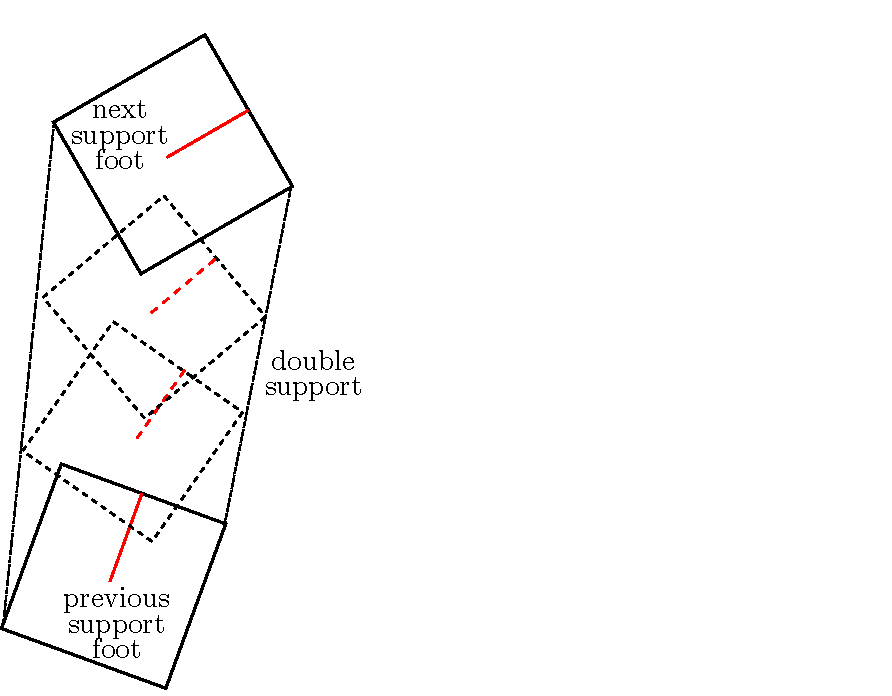
\includegraphics[width=0.3\textwidth]{figures/double_support.pdf}
    \caption{The ZMP constraint moves from a support foot to the following 
        one during double support phase.}
    \label{fig:double-support}
\end{figure}
The expression of the ZMP constraint in 2D can be written as:
\begin{equation}
  \label{eq:zmp-constraint-2d}
  -\frac{1}{2}
  \begin{pmatrix}
    d_x^\text{z} \\
    d_y^\text{z}
  \end{pmatrix}
  \le
  R_{k+i}^T
  \begin{pmatrix}
    x_z^{k+i} - x_f^{k+i} \\
    y_z^{k+i} - y_f^{k+i}
  \end{pmatrix}
  \le
  \frac{1}{2}
  \begin{pmatrix}
    d_x^\text{z} \\
    d_y^\text{z}
  \end{pmatrix}
\end{equation}
where $d_x^\text{z}$ and $d_y^\text{z}$ are the width and the height of the
rectangular constraint region and $R_{k+i}^T$ is the rotation matrix associated
to the orientation $\theta_f^{k+i}$.
Note that $(x_z^{k+i}, y_z^{k+i})$ is the predicted position
of the ZMP, which can be expressed as a linear combination of the control
variables:
\begin{equation}
  \label{eq:piecewise-linear-zmp-trajectory}
  x_z^{k+i} = x_z^k + \delta \sum_{i=0}^{i-1} \dot{x}_z^{k+j}
\end{equation}
Eq. \eqref{eq:zmp-constraint-2d} must be imposed for $i = 1, \dots, N$.

In the 3D case, the ZMP is allowed to leave the ground in order to
generate CoM motions along the $z$ axis as well.
As previously discussed, balance condition requires ZMP to remain inside
polyhedral cone defined by the support polygon and CoM
(Fig. \ref{fig:balance3d}. When ZMP is allowed to move vertically,
the constraint becomes nonlinear. In order to remove nonlinearity it is 
possible to consider a subregion of the polyhedral cone, for example a box
constraint, as shown in Fig. \ref{fig:polyhedral-cone-side-view}:
\begin{equation}
  \label{eq:zmp-constraint-3d}
  -\frac{1}{2}
  \begin{pmatrix}
    \tilde{d}_x^\text{z} \\
    \tilde{d}_y^\text{z} \\
    d_z^\text{z}
  \end{pmatrix}
  \le
  R_{k+i}^T
  \begin{pmatrix}
    x_z^{k+i} - x_f^{k+i} \\
    y_z^{k+i} - y_f^{k+i} \\
    z_z^{k+i} - y_f^{k+i}
  \end{pmatrix}
  \le
  \frac{1}{2}
  \begin{pmatrix}
    \tilde{d}_x^\text{z} \\
    \tilde{d}_y^\text{z} \\
    d_z^\text{z}
  \end{pmatrix}
\end{equation}
where $d_z^\text{z}$ defines the maximum allowed vertical ZMP displacement
with respect to the ground.
To guarantee that the box is contained in the cone, its $x$ and $y$ dimensions 
are respectively reduced to $\tilde{d}_x^\text{z}, \tilde{d}_y^\text{z}$:
\begin{equation}
  \tilde{d}_x^\text{z} = d_x^\text{z} \left( 1 -
      \frac{d_z^\text{z}}{2z_c^{\min}} \right)
      - \frac{d_z^\text{z}}{z_c^{\min}}\Delta x_c
\end{equation}
where $\Delta x_c$ is the maximum expected displacement of the CoM with respect 
to the center of the support foot and $z_c^{\min}$ is the minimum expected
value for CoM height. The same reasoning applies for $\tilde{d}_y^\text{z}$.
\begin{figure}
    \centering
    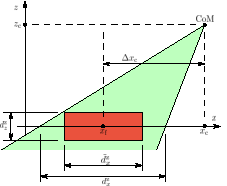
\includegraphics[width=0.7\textwidth]{figures/polyhedral-cone-side-view.pdf}
    \caption{The polyhedral cone representing the ZMP constraint and the 
        box used to approximate the constraint (which becomes linear).}
    \label{fig:polyhedral-cone-side-view}
\end{figure}
Similarly to the 2D case, the box constraint is kept fixed during
single support, while during double support the box 
slides linearly from its position around the previous support foot to its 
position around the next support foot, thus, always remaining within the 
polyhedral cone which defines the ZMP balance constraint, as shown in Fig.
\ref{fig:double-support3D}.
\begin{figure}
    \centering
    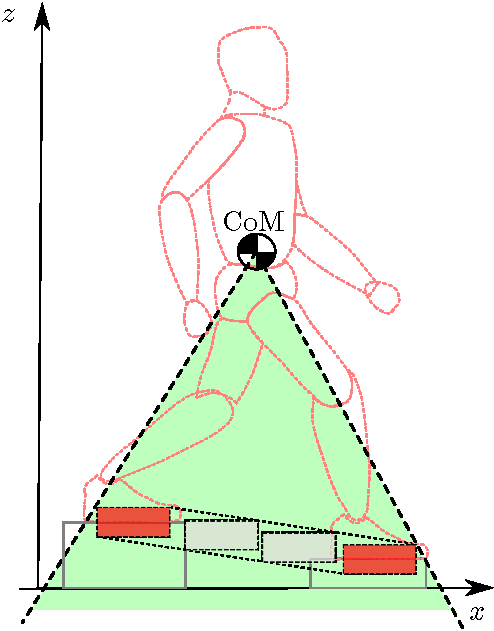
\includegraphics[width=0.5\textwidth]{figures/double_support3D.pdf}
    \caption{The ZMP box constraint moves from a support foot to the following 
        one during double support phase.}
    \label{fig:double-support3D}
\end{figure}
\subsection{Stability constraint}
\label{sec:mpc-stability-constraint}
As previously seen, the motion model
(\ref{eq:com-dynamics-x}-\ref{eq:com-dynamics-z}) is unstable, hence, it is 
not guaranteed that the CoM position is bounded with respect to the ZMP in 
general. This could make the generated gait unrealizable. However, as mentioned 
before and as discussed in \cite{Lanari2014BoundednessII,
DBLP:conf/humanoids/SciancaCSLO16}, it is possible to prove that if the 
initial condition $(x_c^k, \dot{x}_c^k)$ satisfies:
\begin{equation}
  \label{eq:stability-condition-xc}
  x_c^k + \frac{\dot{x}_c^k}{\omega} = \omega \int_{t_k}^\infty 
      e^{-\omega(\tau-t_k)}x_z(\tau)d\tau
\end{equation}
then $x_c$ remains bounded with respect to $x_z$ for
all $t$. An analogous condition can be given for $y_c$ dynamics.
Regarding $z_c$, it is possible to prove its boundedness by using the following
initial condition:
\begin{equation}
  \label{eq:stability-condition-zc}
  z_c^k + \frac{\dot{z}_c^k}{\omega} = \frac{g}{\omega^2} +
      \omega \int_{t_k}^\infty e^{-\omega(\tau-t_k)}z_z(\tau)d\tau
\end{equation}
The above stability conditions can be enforced in the MPC formulation by 
writing them with respect to the control variables $\dot{x}_\text{z}^{k+i},
\dot{y}_\text{z}^{k+i}, \dot{z}_\text{z}^{k+i}$. For $x_c$,
and similarly for $y_c$, the initial condition can be 
writtes as:
\begin{equation}
  \label{eq:stability-constraint-xdot}
  \frac{1}{\omega}\frac{1-e^{-\delta\omega}}{1-e^{-N\delta\omega}}
    \sum_{i=0}^{N-1} e^{-i\delta\omega} \dot{x}_z^{k+i} =
    x_c^k + \frac{\dot{x}_c^k}{\omega} - x_z^k
\end{equation}
which can be obtained from \eqref{eq:stability-condition-xc} by considering 
that the ZMP trajectory \eqref{eq:piecewise-linear-zmp-trajectory} is piecewise 
linear and that the contribution beyond the prediction horizon is computed 
assuming infinite replication of the control variables within the prediction 
horizon itself. A similar initial condition can be written for $z_c$
starting from \eqref{eq:stability-condition-zc}, where $\dot{z}_z$ is set to zero 
beyond the prediction horizon (truncated tail):
\begin{equation}
  \label{eq:stability-constraint-zdot}
  \frac{1-e^{-\delta\omega}}{1-e^{-N\delta\omega}}
    \sum_{i=0}^{N-1} e^{-i\delta\omega} \dot{z}_z^{k+i} =
    z_c^k + \frac{\dot{z}_c^k}{\omega} - z_z^k - \frac{g}{\omega^2}
\end{equation}
A more detailed discussion can be found in
\cite{DBLP:journals/corr/abs-1901-08505}.

\section{MPC Algorithm}
Now that the constraints have been expressed with respect to the input
variables, it is possible to define the MPC scheme used to generate the gait.
In particular, the MPC algorithm solves a QP problem at each iteration
determining the trajectory of the CoM. Note that the footsteps are assigned in 
advance.

Considering the decision variable vectors:
\begin{align}
  \dot{X}_\text{z}^k&=(\dot{x}_\text{z}^k, \dots, \dot{x}_\text{z}^{k+N-1})^T \\
  \dot{Y}_\text{z}^k&=(\dot{y}_\text{z}^k, \dots, \dot{y}_\text{z}^{k+N-1})^T \\
  \dot{Z}_\text{z}^k&=(\dot{z}_\text{z}^k, \dots, \dot{z}_\text{z}^{k+N-1})^T
\end{align}
the QP problem can be defined as:
\begin{align*}
  \min_{\dot{X}_\text{z}^k, \dot{Y}_\text{z}^k, \dot{Z}_\text{z}^k}
      &\sum_{i=1}^N
      \biggl[
          (\dot{x}_z^{k+i})^2 +
          (\dot{y}_z^{k+i})^2 +
          (\dot{z}_z^{k+i})^2 + \\
          &\beta \biggl(
              (x_z^{k+i} - x_f^{k+i})^2 +
              (y_z^{k+i} - y_f^{k+i})^2 +
              (z_z^{k+i} - z_f^{k+i})^2
          \biggr)
      \biggr]\\
      \textrm{s.t. } &\textrm{ZMP constraint \eqref{eq:zmp-constraint-3d}} \\
      &\textrm{stability constraints \eqref{eq:stability-constraint-xdot},
          \eqref{eq:stability-constraint-zdot}}
\end{align*}
where the cost function includes the decision variables for regularization 
purposes and a term which attempts to bring the ZMP to the center of the 
footstep.

Each MPC iteration starts at $t_k$ and executes the steps described in Algorithm
\ref{algo:mpc-iteration}, defining the trajectory of the CoM.
\begin{algorithm}
\SetAlgoLined
\KwResult{CoM trajectory}
  Compute $\dot{X}_\text{z}^k$, $\dot{Y}_\text{z}^k$, $\dot{Z}_\text{z}^k$ 
      that solve the QP problem\;
  From the solutions, extract the first control samples
      $\dot{x}_\text{z}^k$, $\dot{y}_\text{z}^k$, $\dot{z}_\text{z}^k$\;
  Set $\dot{x}_z=\dot{x}_\text{z}^k$ in \eqref{eq:vhcomlip-motion-model}
      and integrate from $(x_c^k, \dot{x}_c^k, x_\text{z}^k)$ to obtain 
      $x_c(t)$, $\dot{x}_c(t)$, $x_\text{z}(t)$ for
      $t \in [t_k, t_{k+1}]$. The same applies for for $y$, $z$.
  \caption{MPC iteration}
  \label{algo:mpc-iteration}
\end{algorithm}

\section{BHuman Implementation}
The MPC scheme has been implemented in C++ upon the BHuman framework
\cite{BHumanCodeRelease2018} and it has been tested on both dynamic environments 
and NAO humanoid robot. The QP problem has been solved using qpOASES
\cite{qpOASES}. The footstep plan is either generated by the footstep planner 
described in Chapter \ref{ch:rrt-based-footstep-planning} or manually assigned 
before the execution of the program. Experiments are described in detail in 
Chapter \ref{ch:experiments}. Note that to speed up the execution of the code 
in order to keep computation within the sampling time of the kinematic 
controller, the rotation matrix of the ZMP constraint described in Eq.
\eqref{eq:zmp-constraint-3d} has been neglected. This does not create any
problem if the size of the box is small enough to stay within the poyhedral 
cone regardless of the rotation of the feet. The MPC hyperparameters have been 
set in the following way: $\omega=6.68 {\rm s}^{-1}$,
the step duration $T_s=0.48 {\rm s}$ of which $t_{\rm SS}=0.30 {\rm s}$ of
single support and 
$t_{\rm DS}=0.18 {\rm s}$ of double support. The size of the box constraint have 
been set to $\tilde{d}_x^{\rm z}=0.05 {\rm m}, \tilde{d}_y^{\rm z}=0.05 {\rm m},
\tilde{d}_z^{\rm z}=0.05 {\rm m}$.


\chapter{Experiments}
\label{ch:experiments}
\section{NAO}
Brief description of NAO v5 (which is running BHuman).

\section{Simple Staircase}
Staircase from 1cm to 5cm. Limitations of the robot.
\begin{figure}
  \centering
  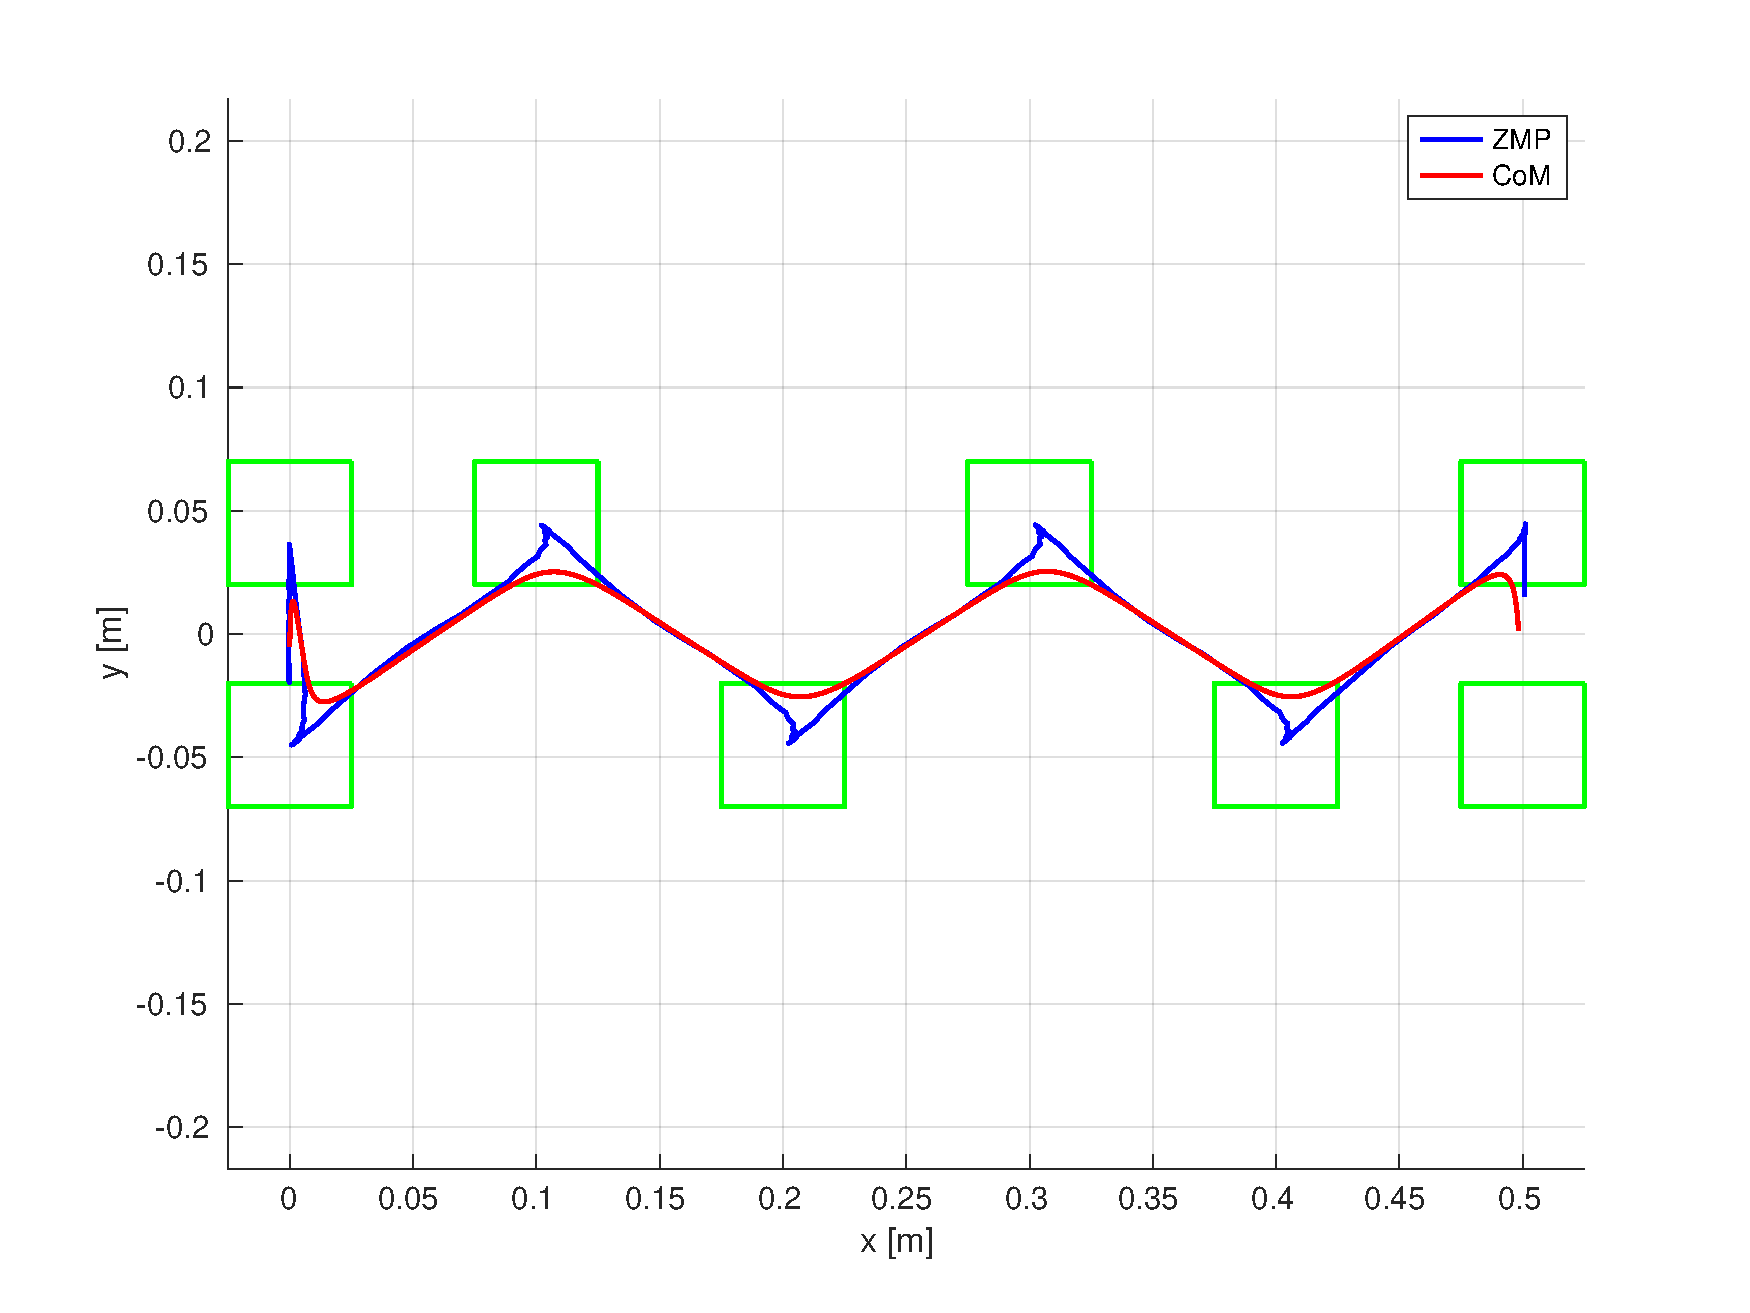
\includegraphics[width=\textwidth]
      {figures/experiments/simple-staircase/xy-plot-4cm.pdf}
  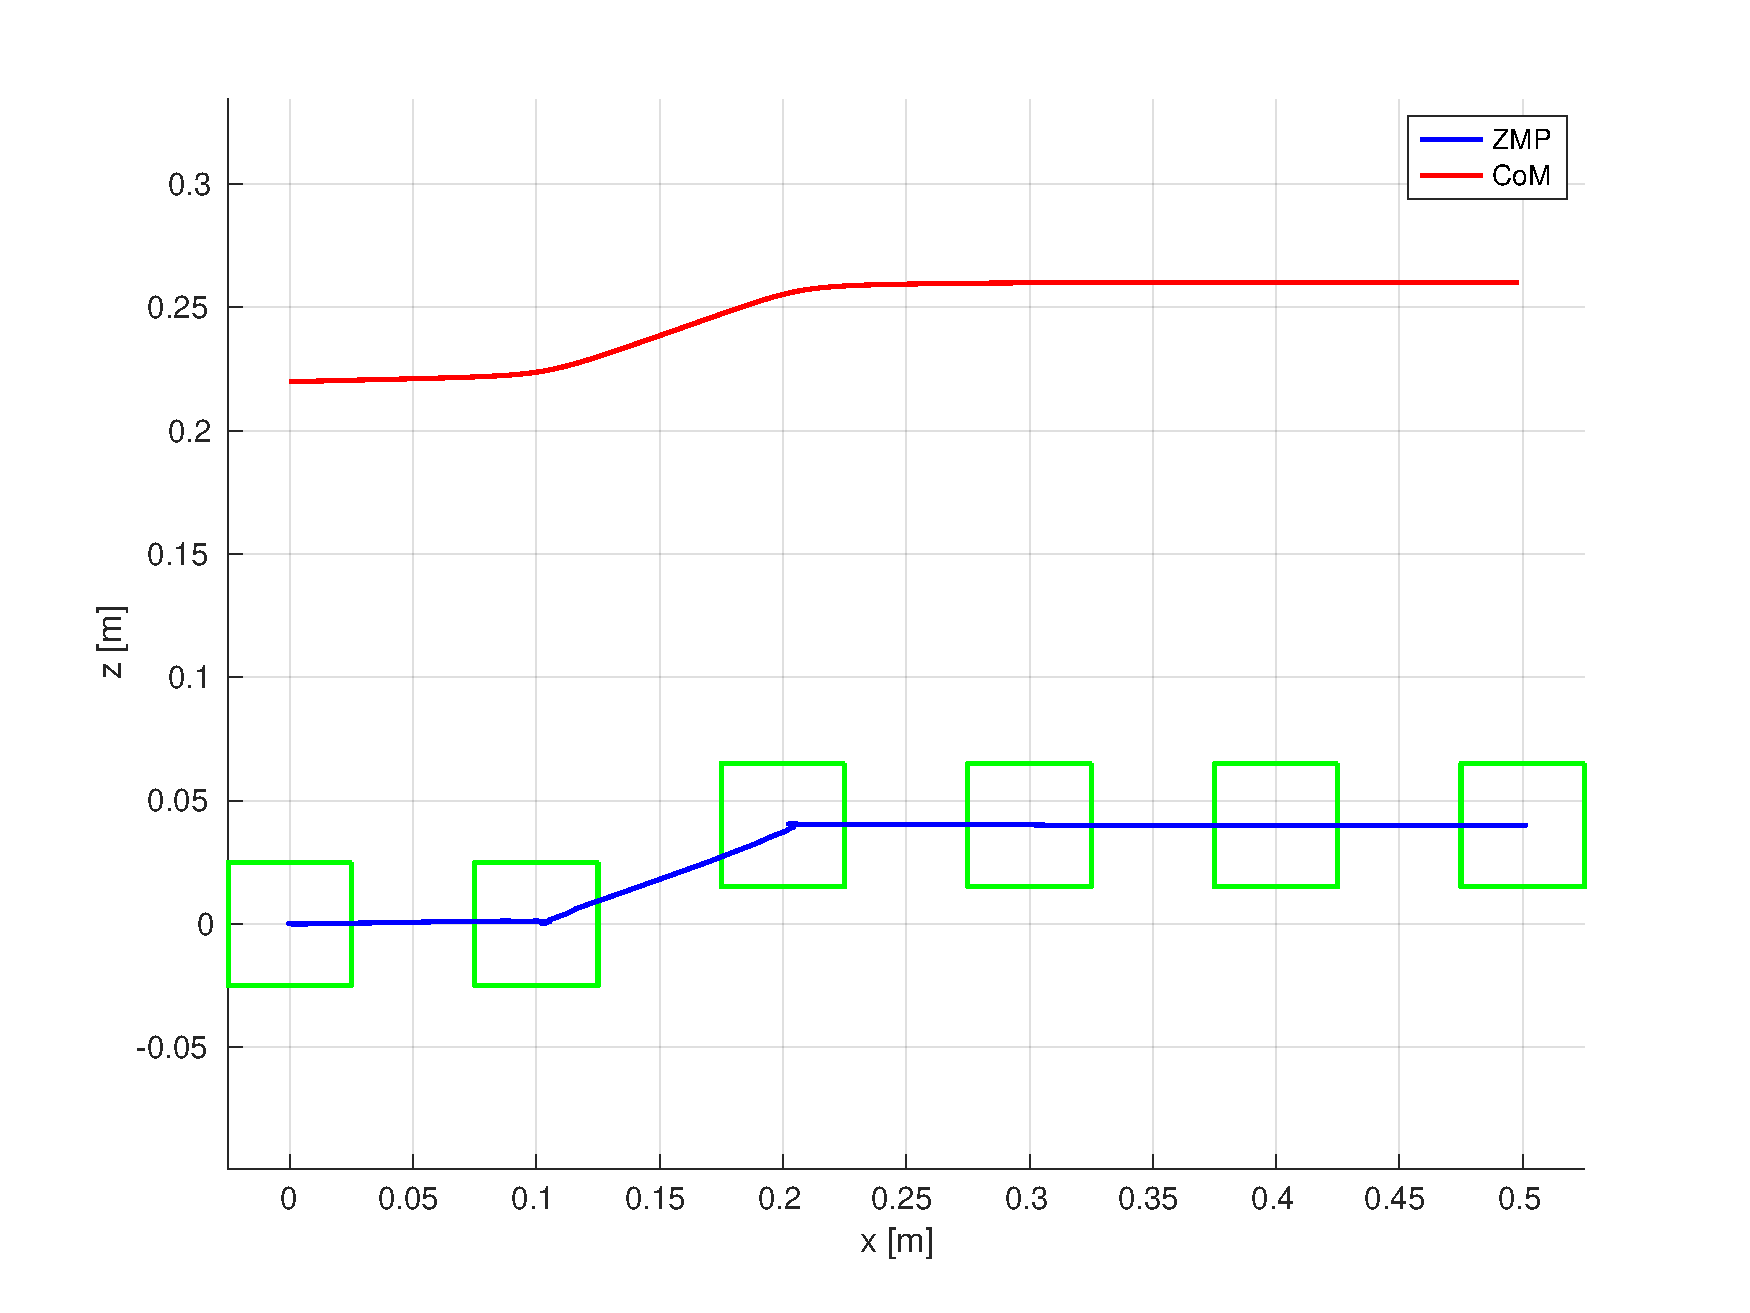
\includegraphics[width=\textwidth]
      {figures/experiments/simple-staircase/xz-plot-4cm.pdf}
  \caption{The plots show how the CoM and the ZMP vary with respect to the
		footsteps in the scenario ``Simple Staircase''.
    The green boxes represent the footsteps.}
  \label{fig:experiments:simple-staircase:comzmp}
\end{figure}

\section{Multiple Staircases}
Two consecutive staircases of 2cm.

\subsection{Upstairs}
Upstairs.
\begin{figure}
  \begin{subfigure}{0.48\textwidth}
    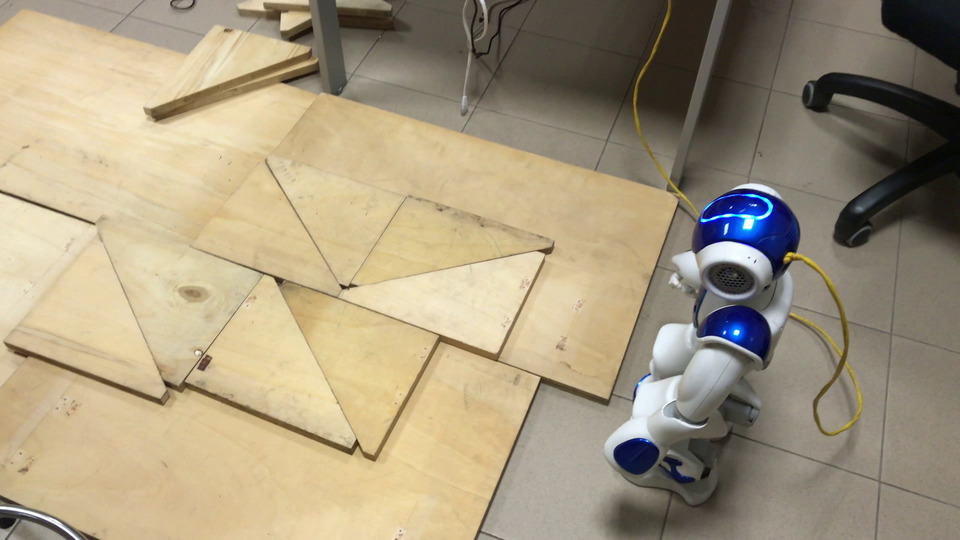
\includegraphics[width=\linewidth]
      {figures/experiments/multiple-staircases/upstairs/video/01.png}
    \caption{Starting position}
    \label{fig:exp:ms:up:frame1}
  \end{subfigure}\hspace*{\fill}
  \begin{subfigure}{0.48\textwidth}
    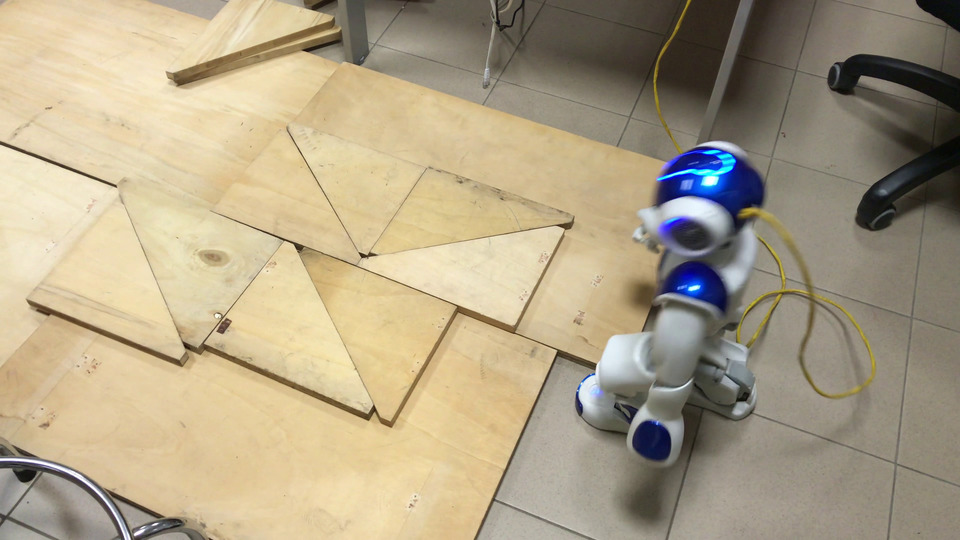
\includegraphics[width=\linewidth]
      {figures/experiments/multiple-staircases/upstairs/video/02.png}
    \caption{First step}
  \end{subfigure}
  \begin{subfigure}{0.48\textwidth}
    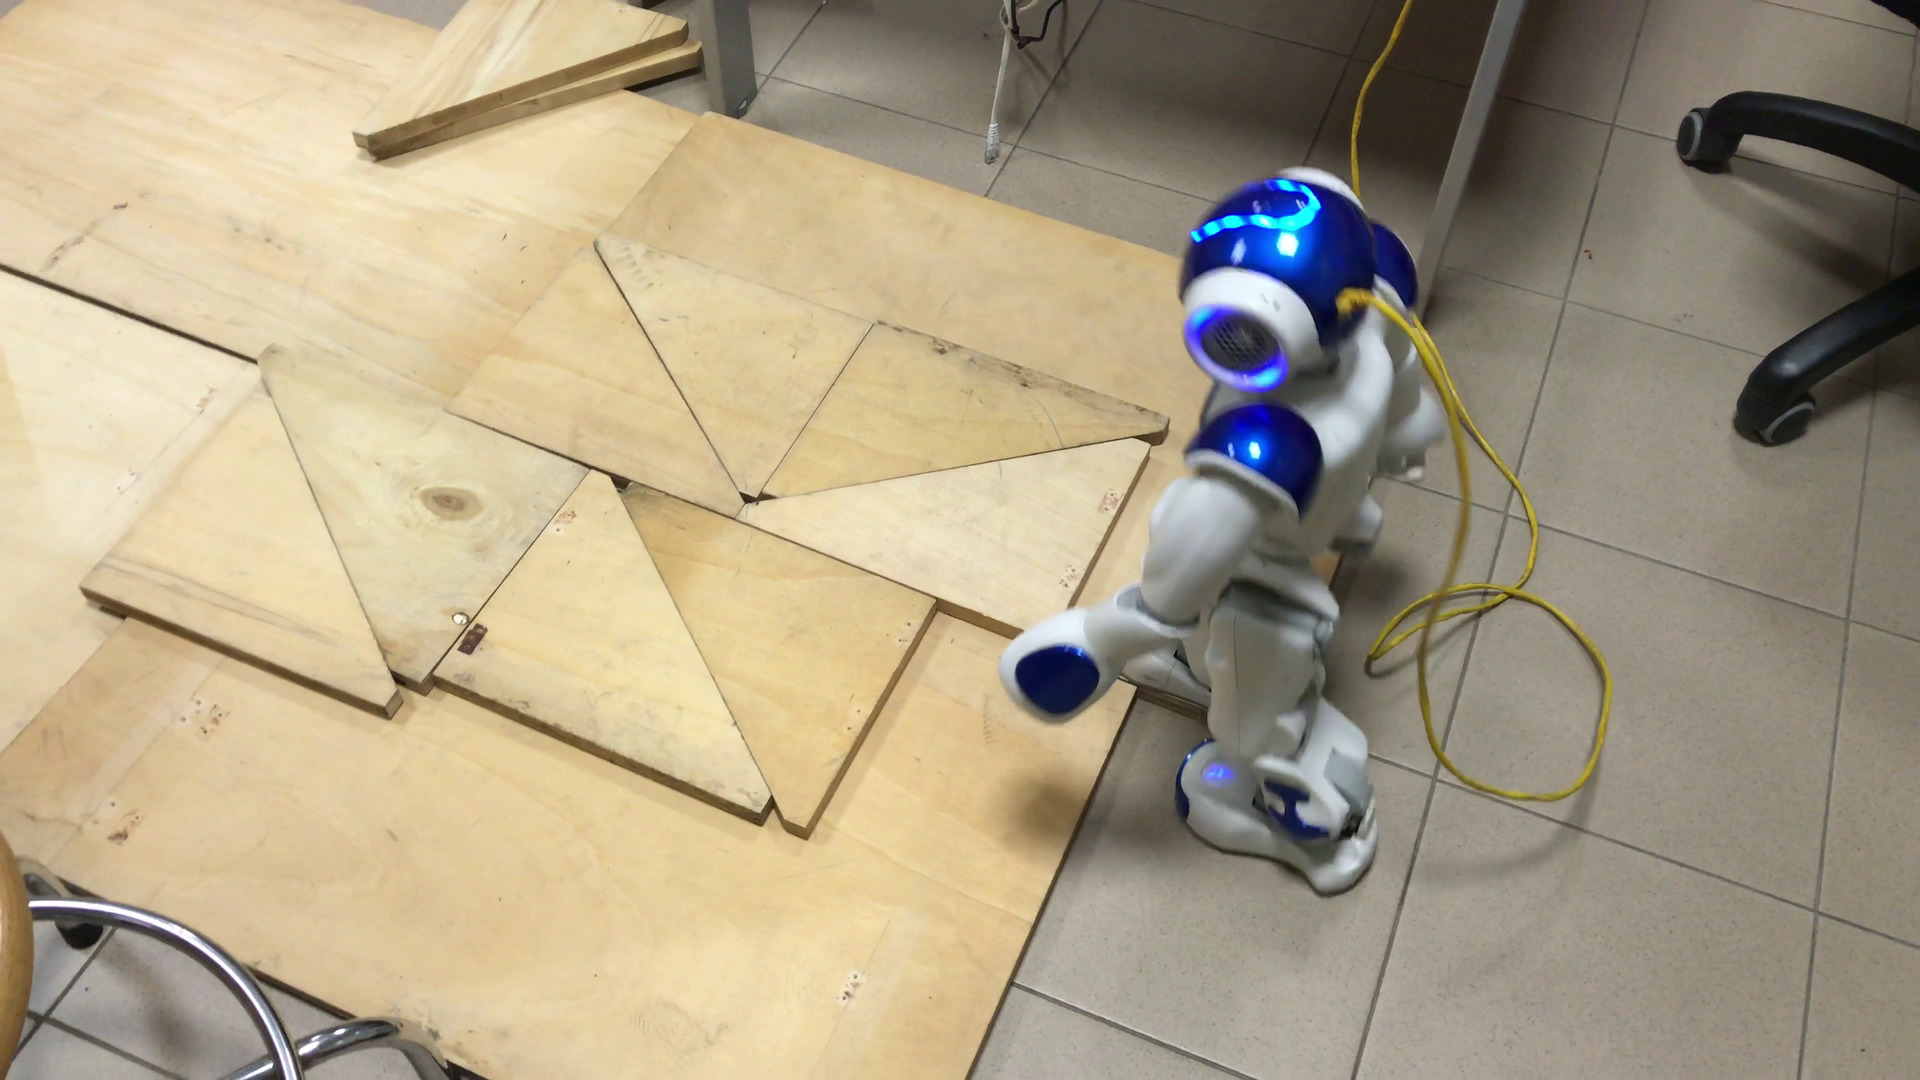
\includegraphics[width=\linewidth]
      {figures/experiments/multiple-staircases/upstairs/video/03.png}
    \caption{Second step}
  \end{subfigure}\hspace*{\fill}
  \begin{subfigure}{0.48\textwidth}
    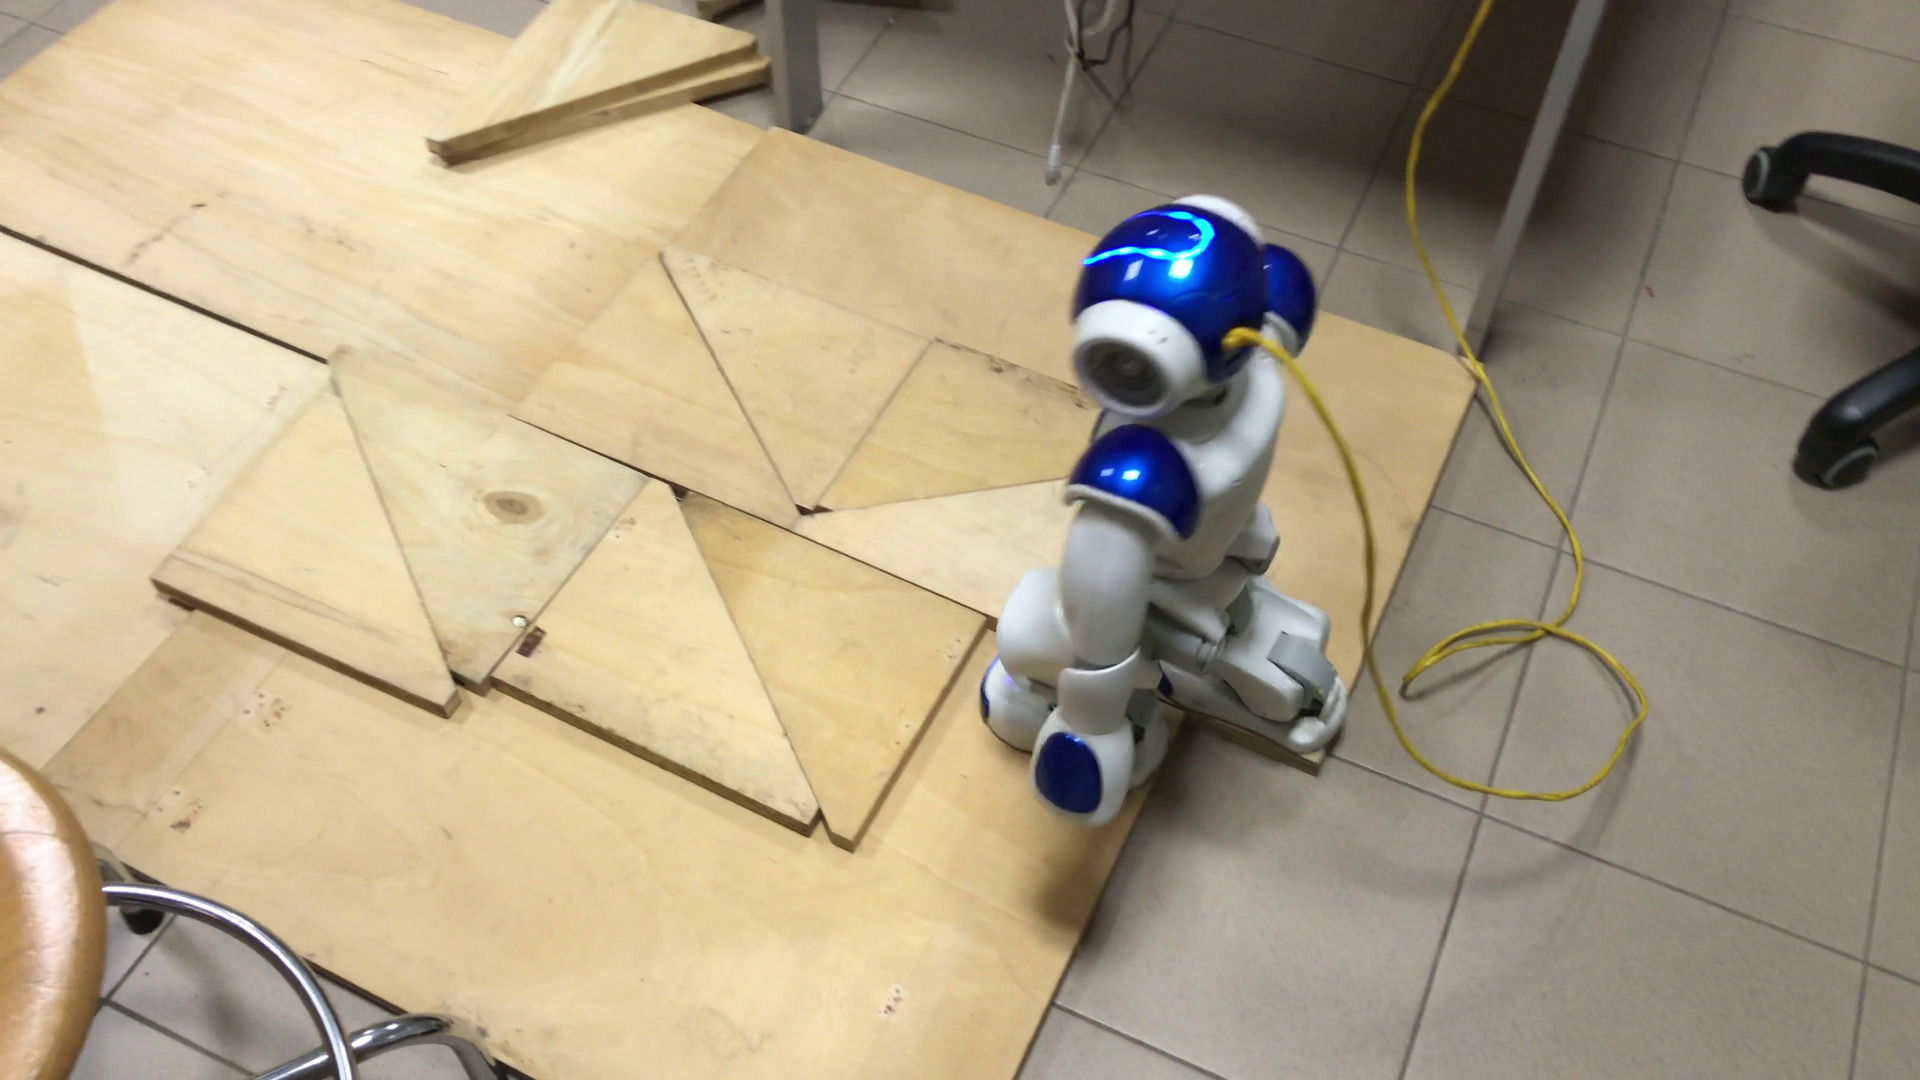
\includegraphics[width=\linewidth]
      {figures/experiments/multiple-staircases/upstairs/video/04.png}
    \caption{Third step}
  \end{subfigure}
  \begin{subfigure}{0.48\textwidth}
    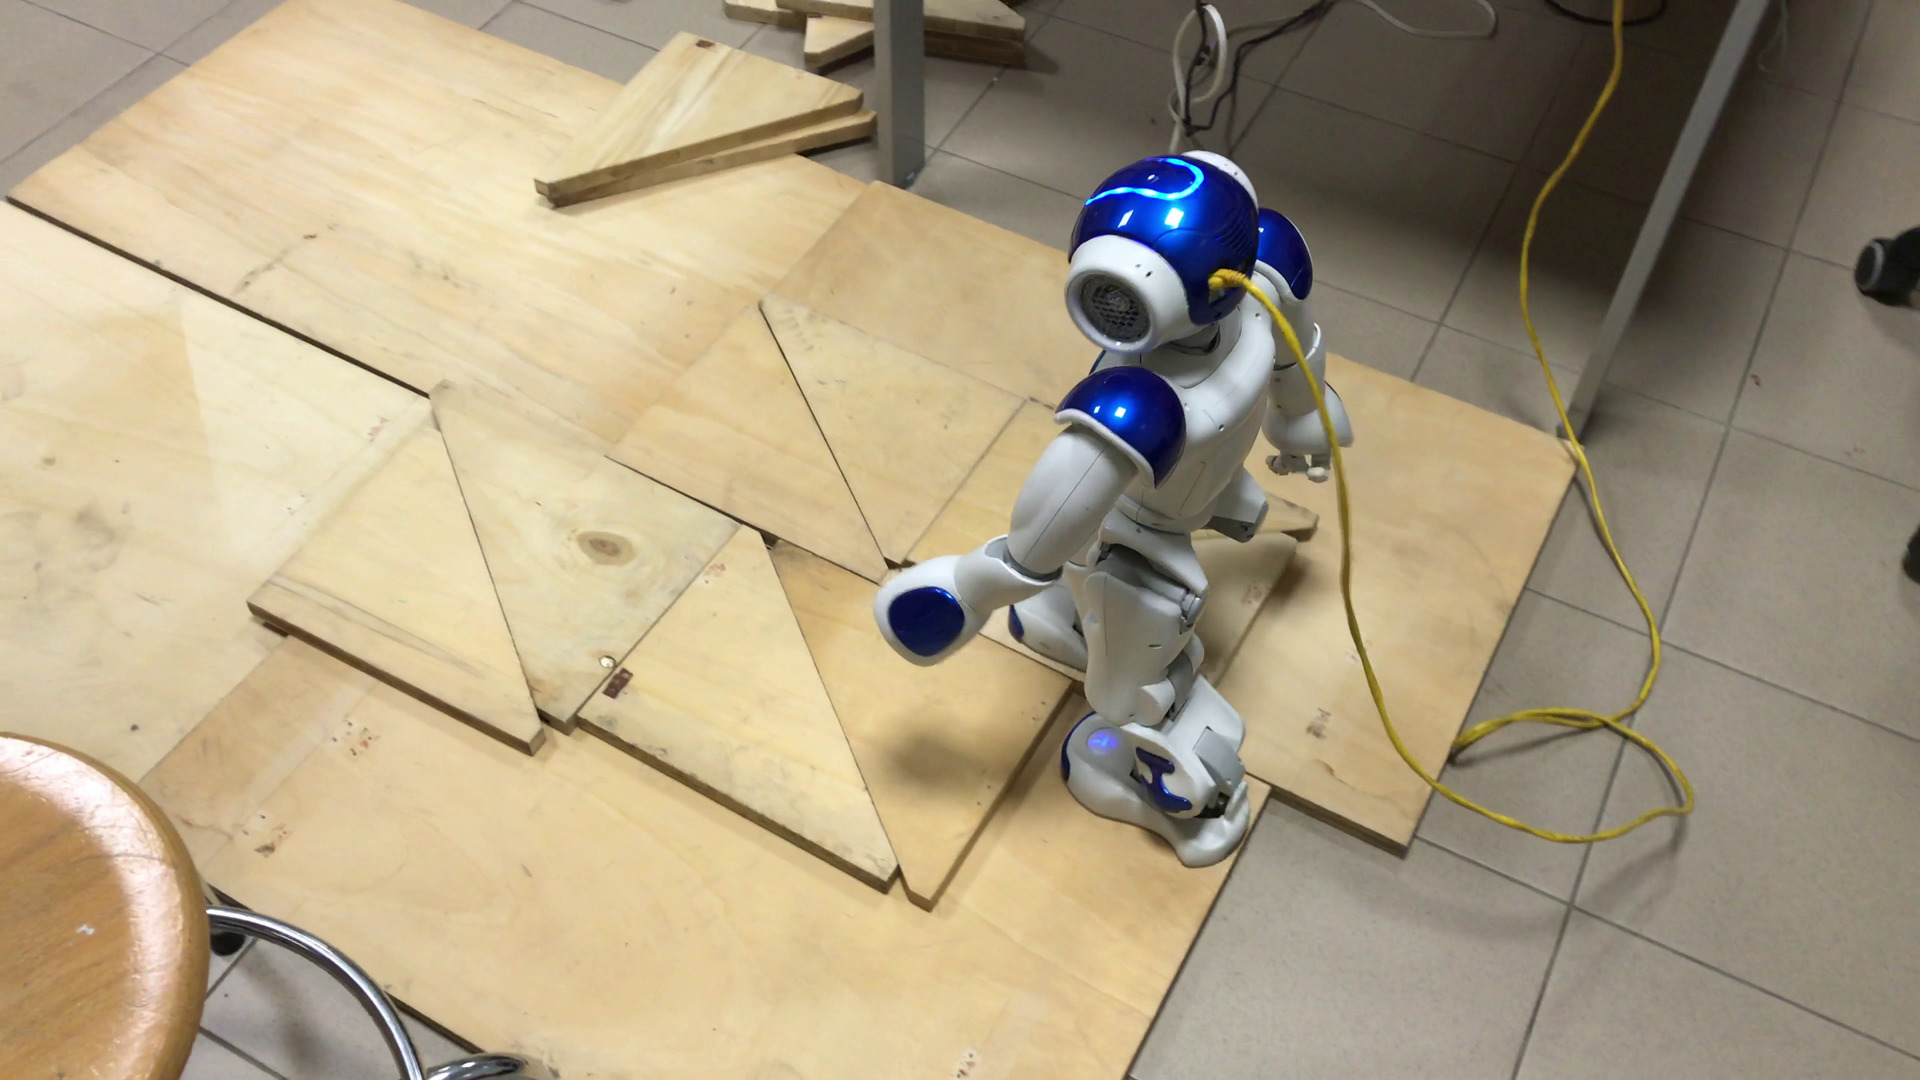
\includegraphics[width=\linewidth]
      {figures/experiments/multiple-staircases/upstairs/video/05.png}
    \caption{Fourth step}
  \end{subfigure}\hspace*{\fill}
  \begin{subfigure}{0.48\textwidth}
    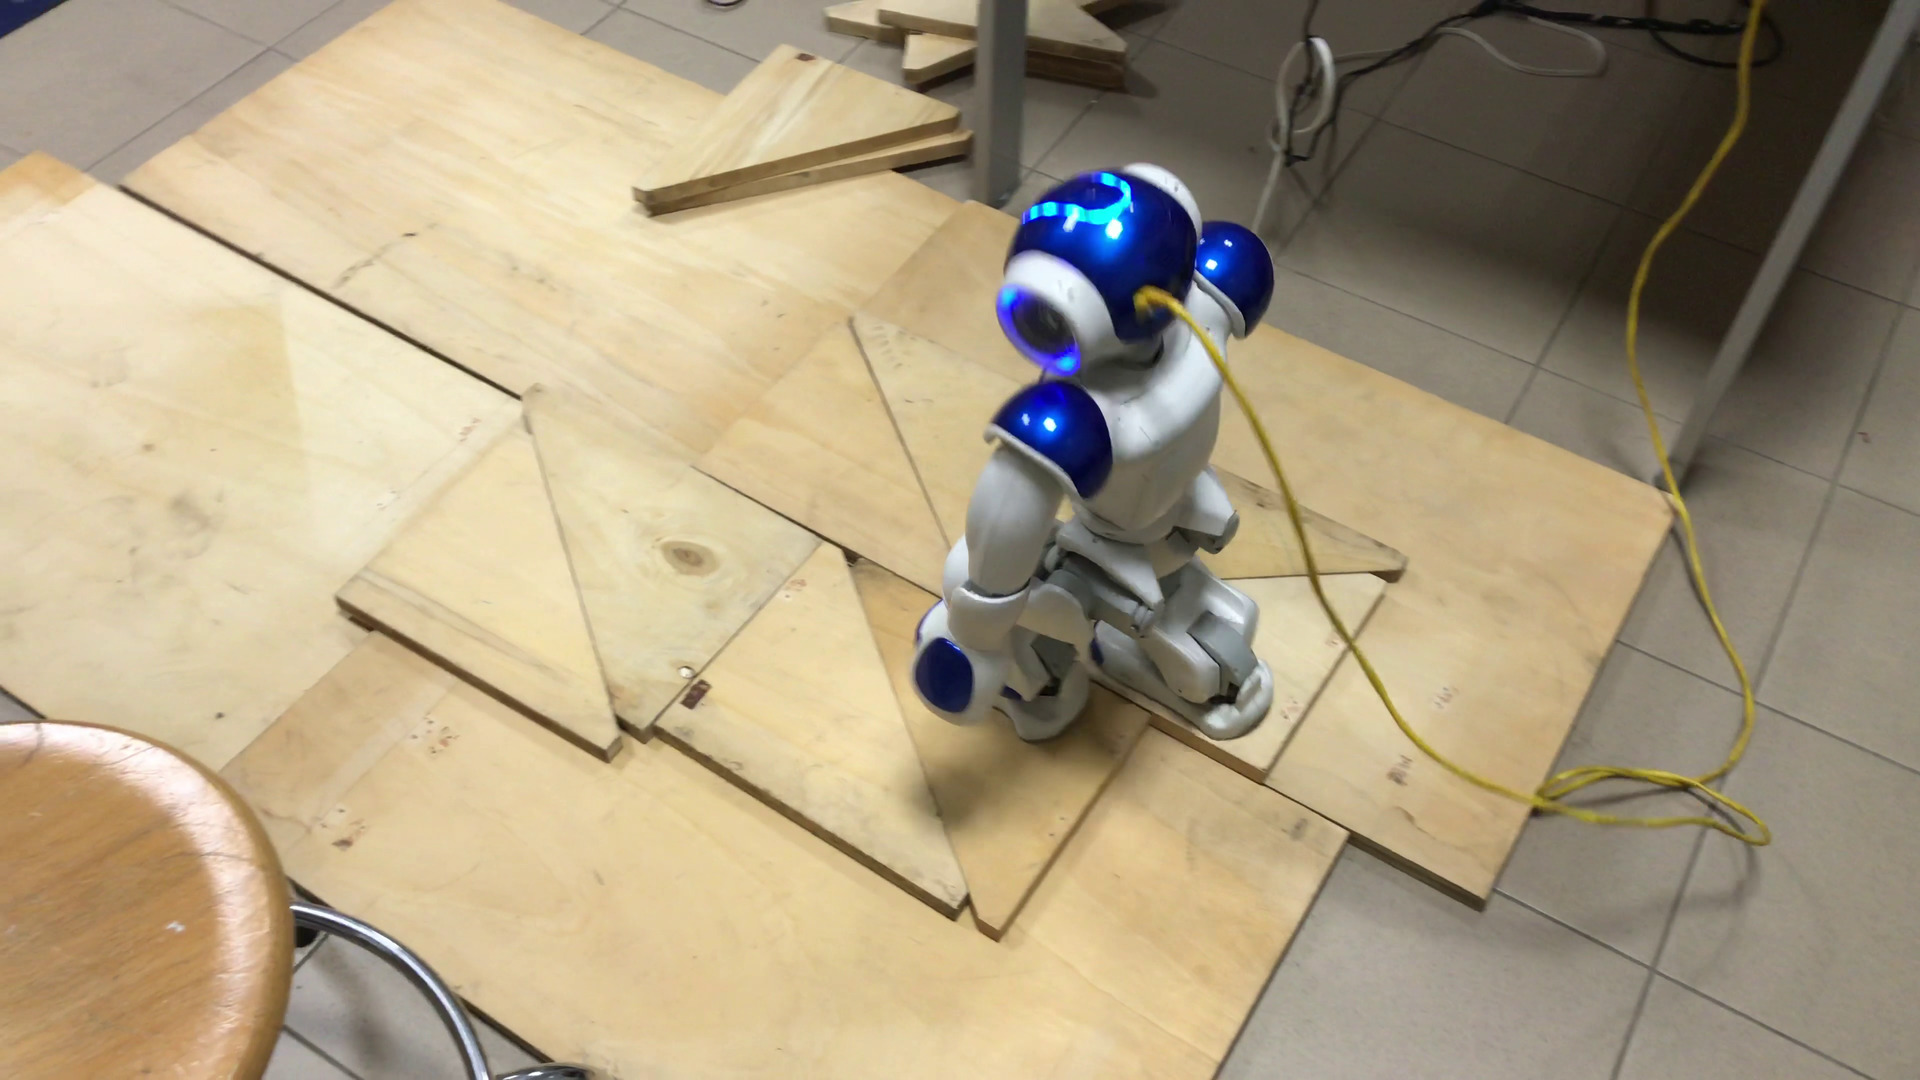
\includegraphics[width=\linewidth]
      {figures/experiments/multiple-staircases/upstairs/video/06.png}
    \caption{Fifth step}
  \end{subfigure}
  \caption{The figures show the motion of the robot for the scenario
      ``Multiple Staircases (Upstairs)''. The robot starts just in 
      front of the stairs (Fig. \ref{fig:exp:ms:up:frame1}), then it places 
      each step one in front of the other without colliding with the staircases,
      safely climbing the stairway. Each staircase has a height of 2 cm.}
  \label{fig:experiments:multiple-staircases:upstairs:videoframes}
\end{figure}

\begin{figure}
  \centering
  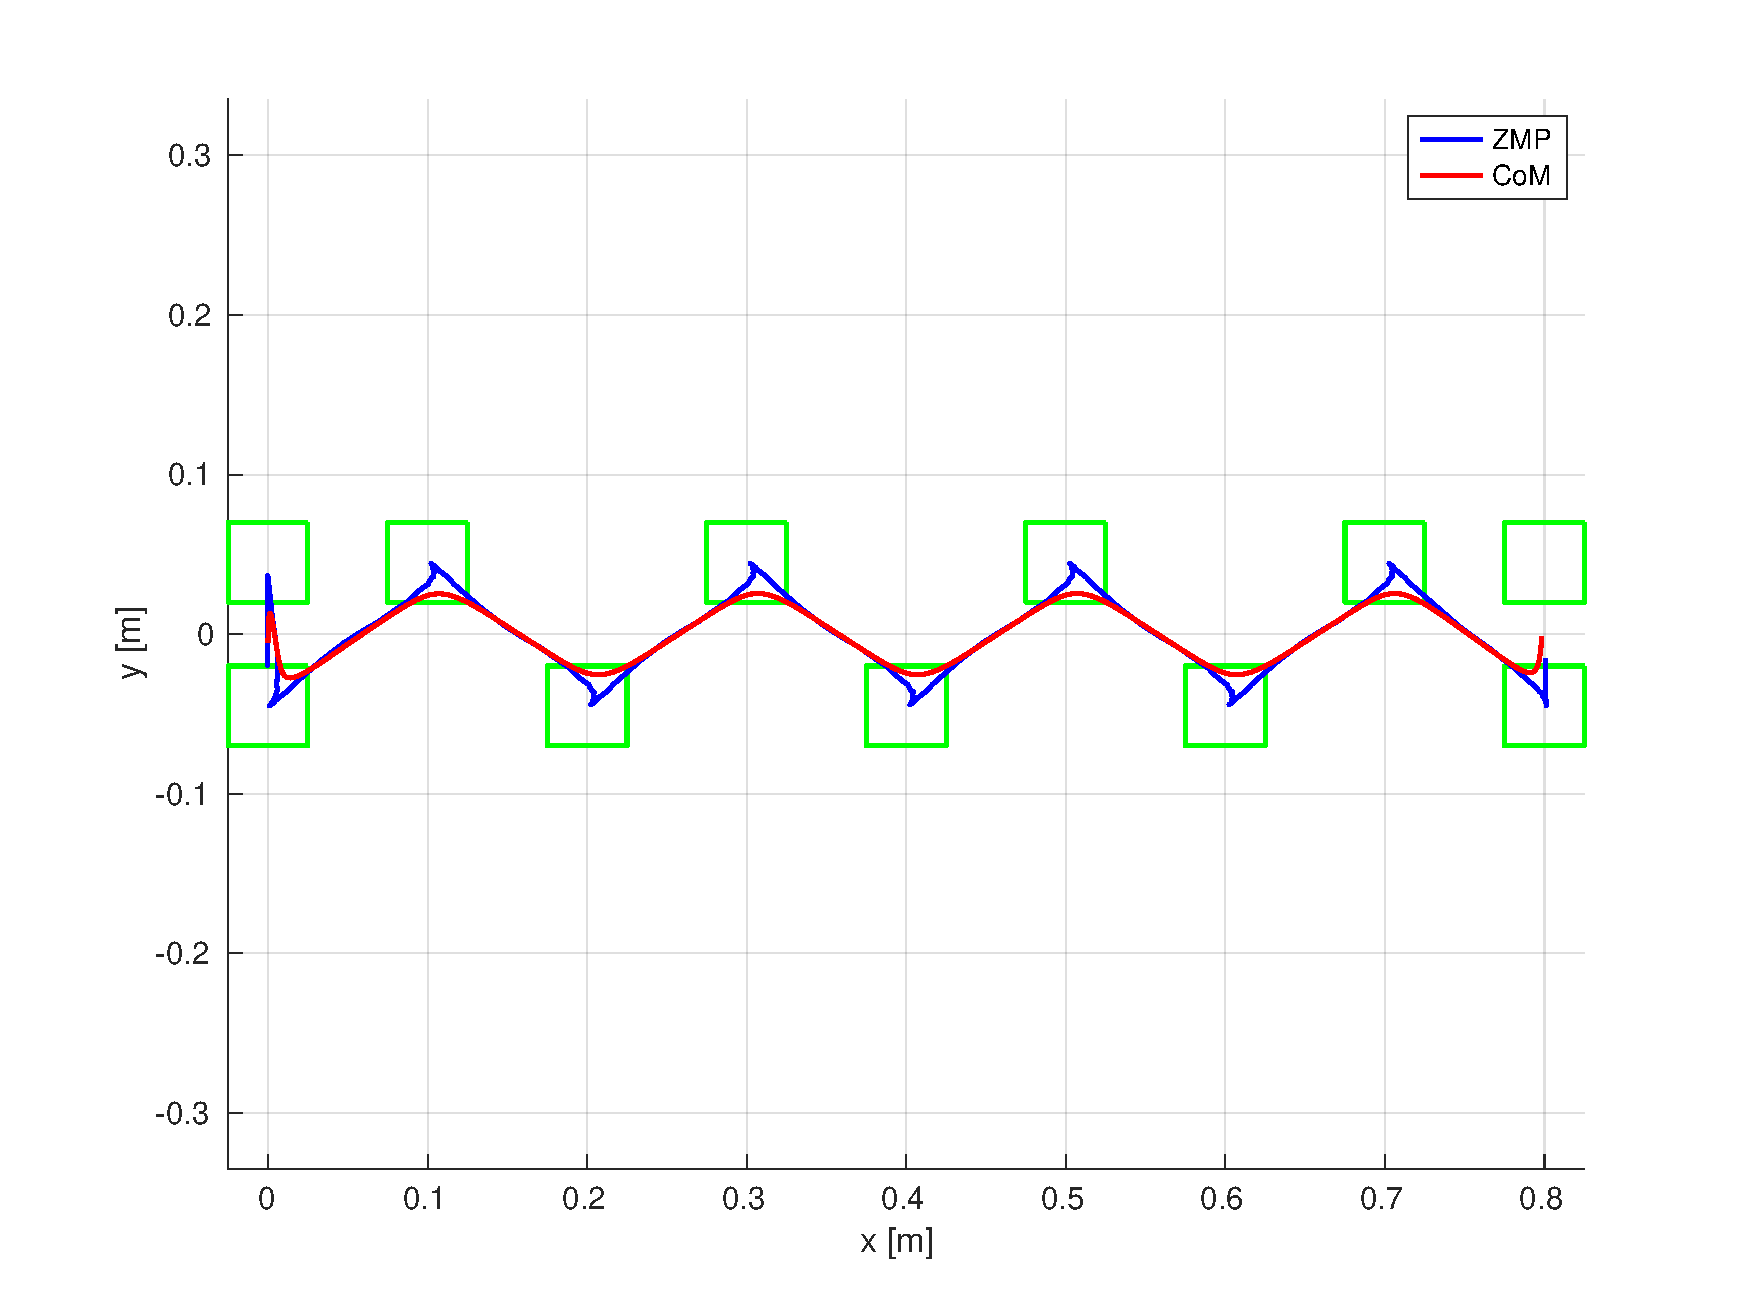
\includegraphics[width=\textwidth]
      {figures/experiments/multiple-staircases/upstairs/xy-plot-2cm.pdf}
  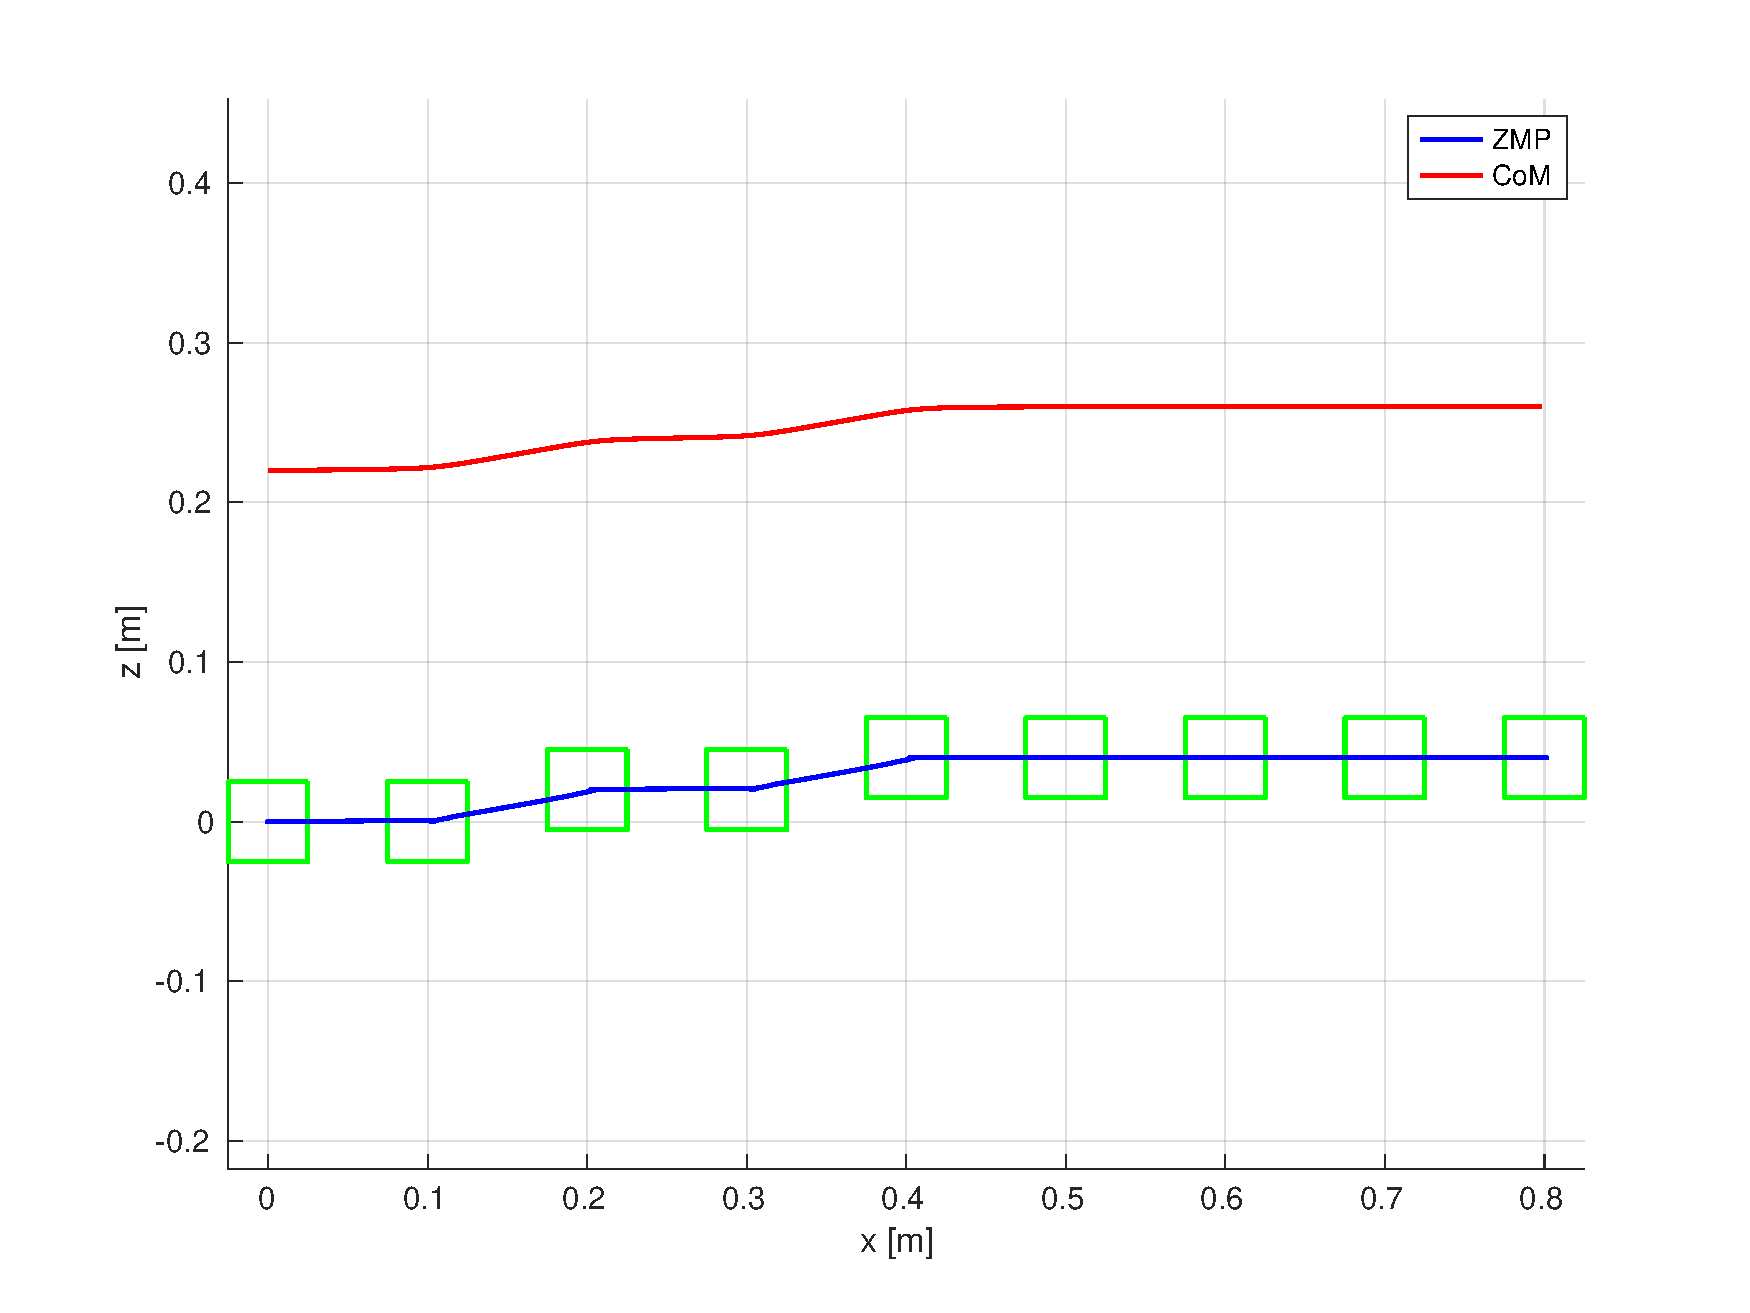
\includegraphics[width=\textwidth]
      {figures/experiments/multiple-staircases/upstairs/xz-plot-2cm.pdf}
  \caption{The plots show how the CoM and the ZMP vary with respect to the
		footsteps in the scenario ``Multiple Staircases (Upstairs)''.
    The green boxes represent the footsteps.}
  \label{fig:experiments:multiple-staircases:upstairs:comzmp}
\end{figure}

\subsection{Downstairs}
Downstairs.
\begin{figure}
  \begin{subfigure}{0.48\textwidth}
    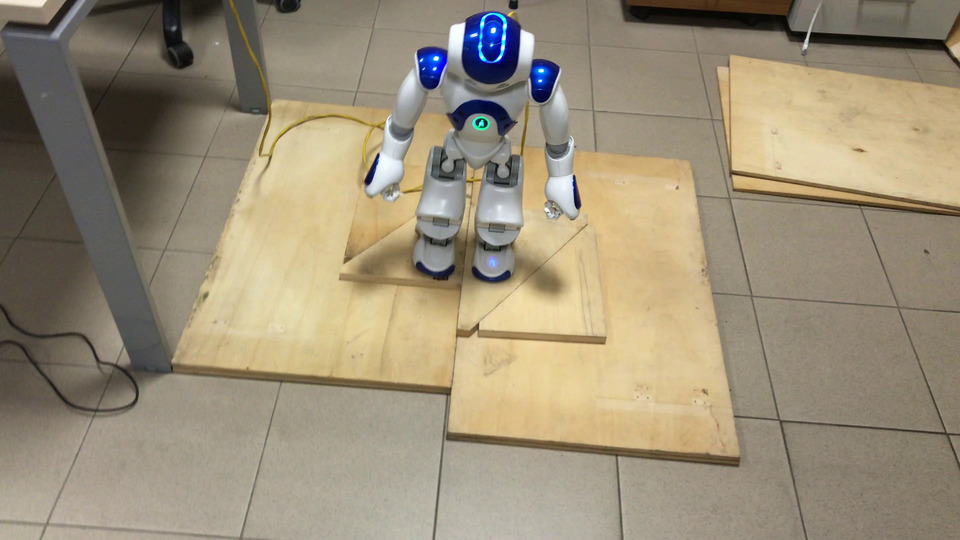
\includegraphics[width=\linewidth]
      {figures/experiments/multiple-staircases/downstairs/video/01.png}
    \caption{Starting position}
    \label{fig:exp:ms:down:frame1}
  \end{subfigure}\hspace*{\fill}
  \begin{subfigure}{0.48\textwidth}
    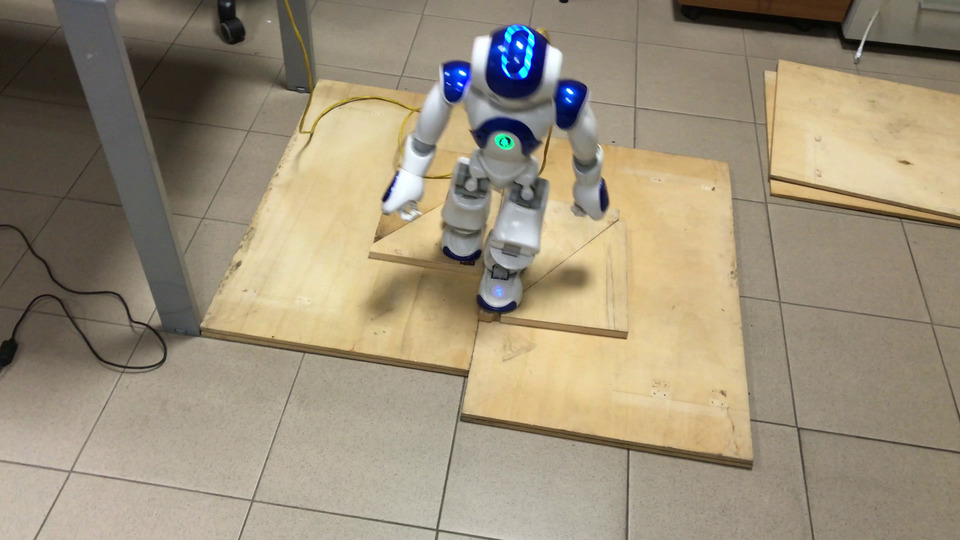
\includegraphics[width=\linewidth]
      {figures/experiments/multiple-staircases/downstairs/video/02.png}
    \caption{First step}
  \end{subfigure}
  \begin{subfigure}{0.48\textwidth}
    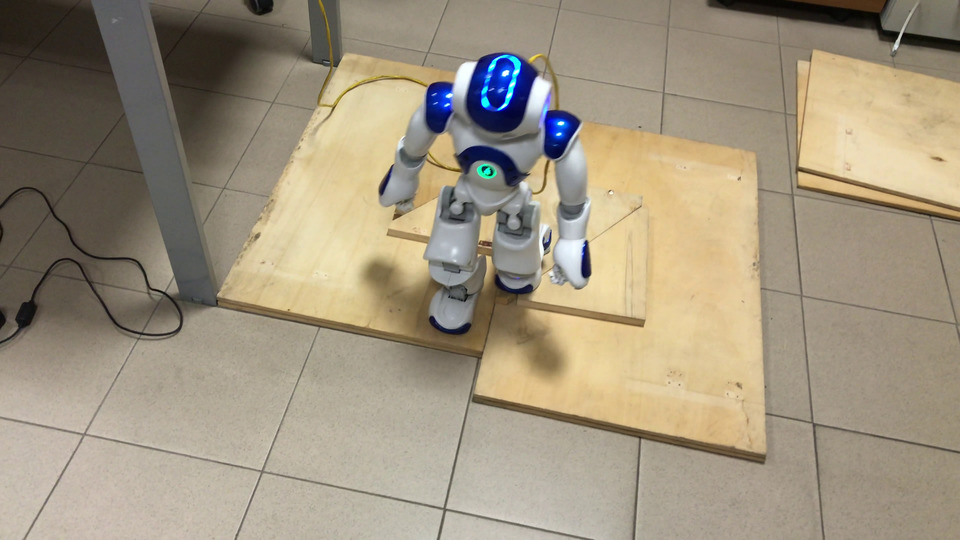
\includegraphics[width=\linewidth]
      {figures/experiments/multiple-staircases/downstairs/video/03.png}
    \caption{Second step}
  \end{subfigure}\hspace*{\fill}
  \begin{subfigure}{0.48\textwidth}
    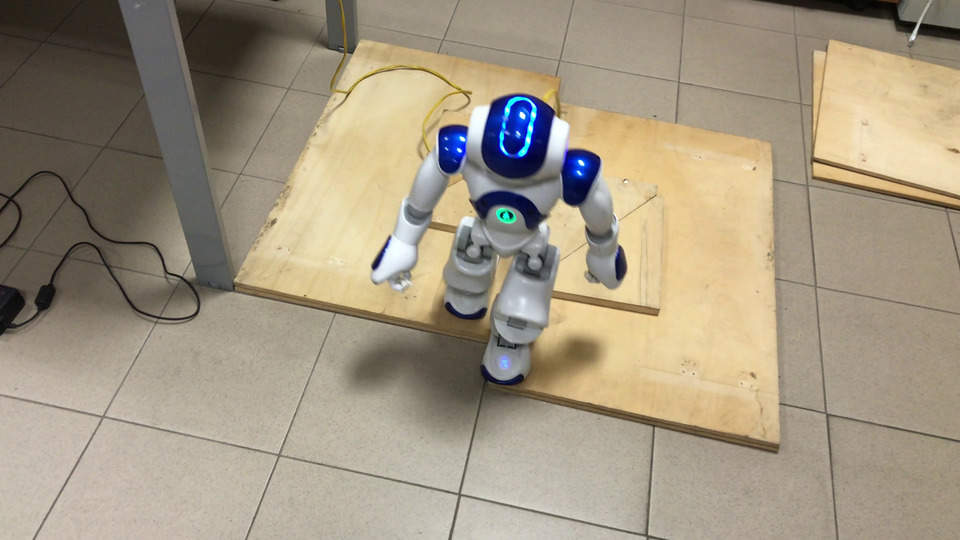
\includegraphics[width=\linewidth]
      {figures/experiments/multiple-staircases/downstairs/video/04.png}
    \caption{Third step}
  \end{subfigure}
  \begin{subfigure}{0.48\textwidth}
    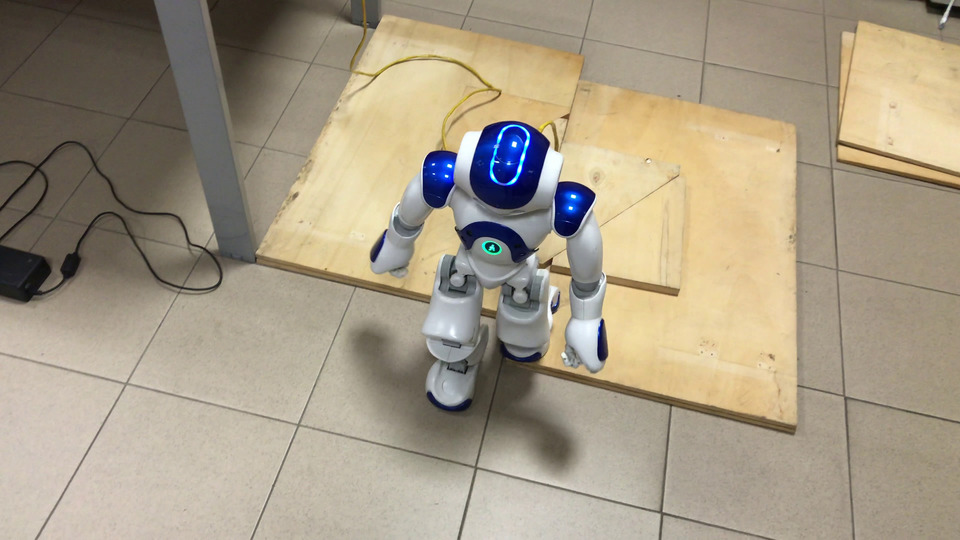
\includegraphics[width=\linewidth]
      {figures/experiments/multiple-staircases/downstairs/video/05.png}
    \caption{Fourth step}
  \end{subfigure}\hspace*{\fill}
  \begin{subfigure}{0.48\textwidth}
    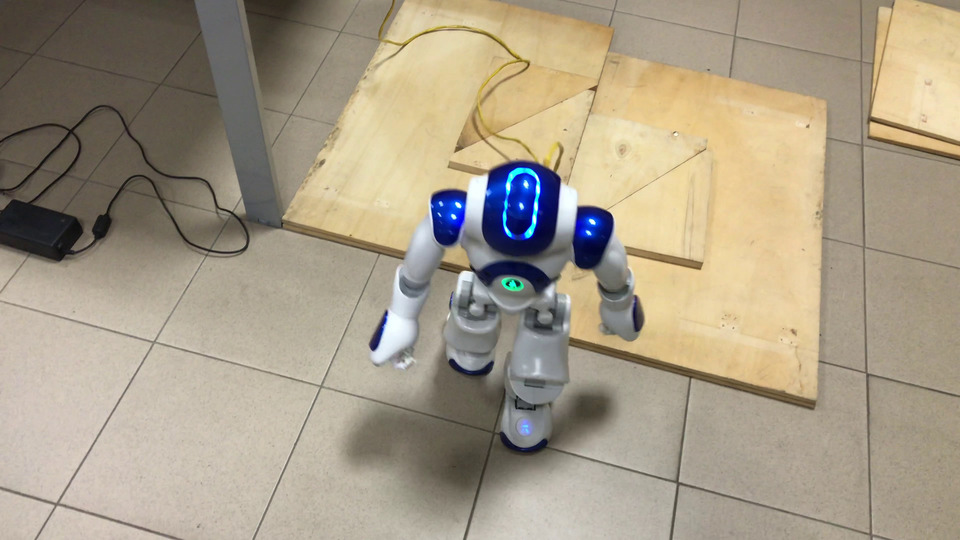
\includegraphics[width=\linewidth]
      {figures/experiments/multiple-staircases/downstairs/video/06.png}
    \caption{Fifth step}
  \end{subfigure}
  \caption{The figures show the motion of the robot for the scenario
      ``Multiple Staircases (Downstairs)''. The robot starts on top of the 
      stairway (Fig. \ref{fig:exp:ms:down:frame1}), then it places 
      each step one in front of the other without colliding with the staircases,
      safely reaching ground level. Each staircase has a height of 2 cm.}
  \label{fig:experiments:multiple-staircases:downstairs:videoframes}
\end{figure}

\begin{figure}
  \centering
  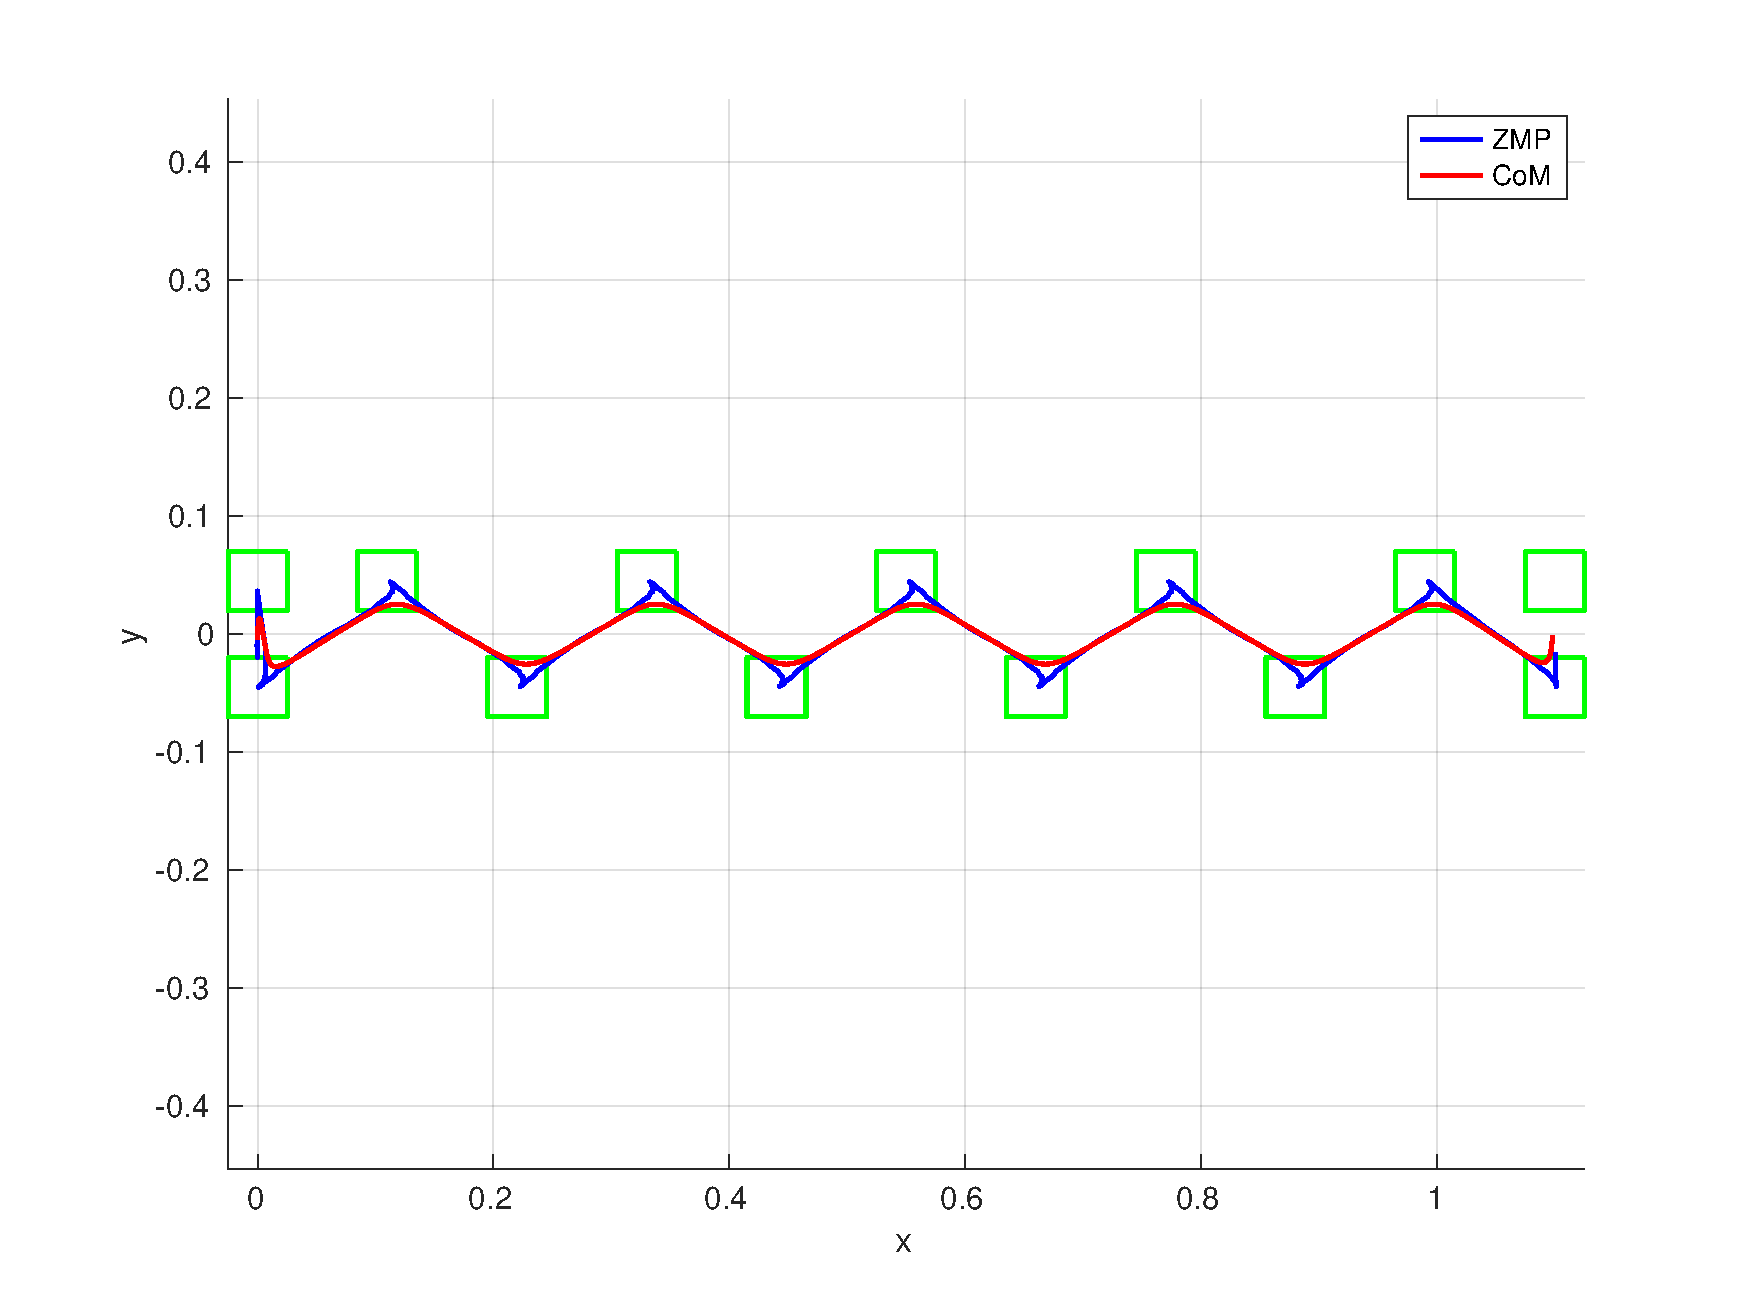
\includegraphics[width=\textwidth]
      {figures/experiments/multiple-staircases/downstairs/xy-plot-2cm.pdf}
  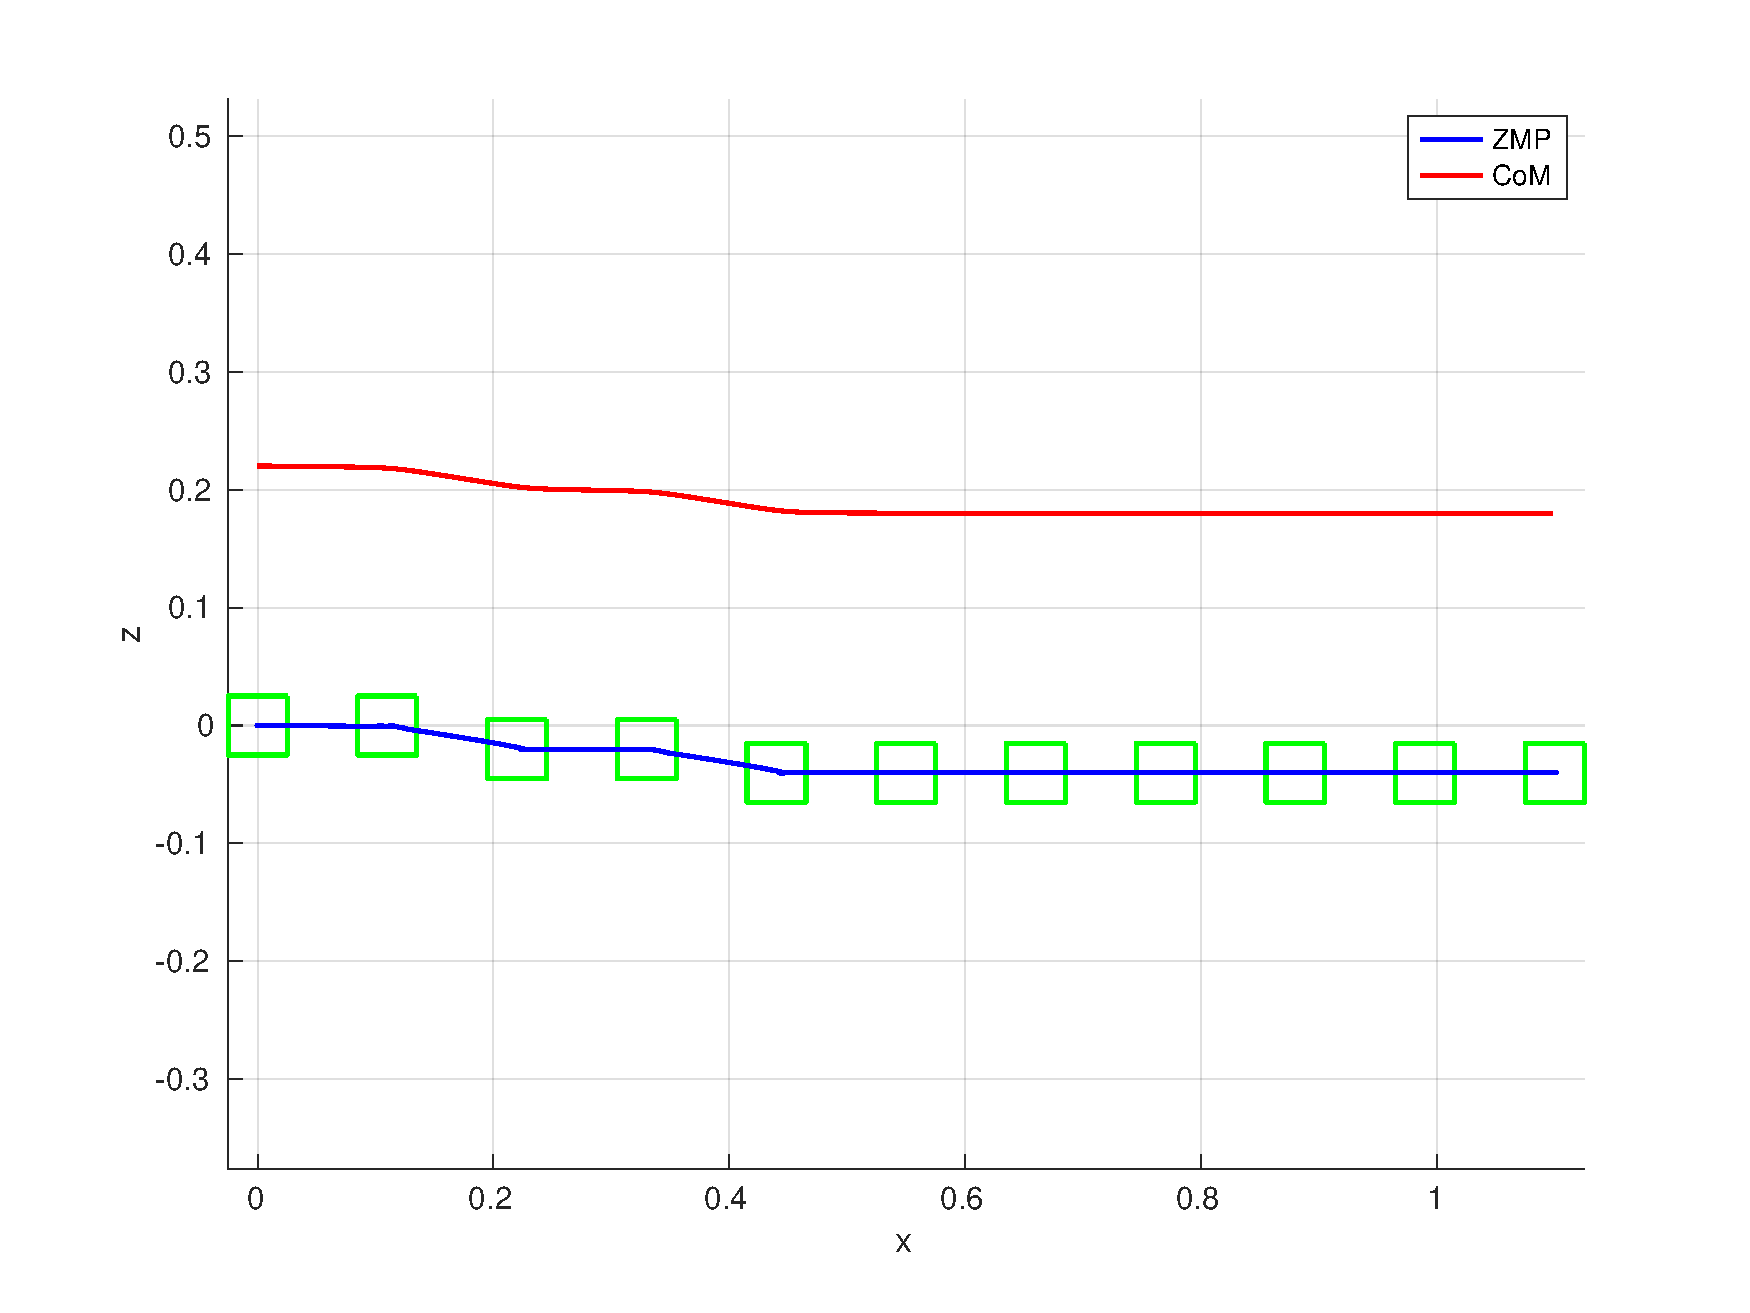
\includegraphics[width=\textwidth]
      {figures/experiments/multiple-staircases/downstairs/xz-plot-2cm.pdf}
  \caption{The plots show how the CoM and the ZMP vary with respect to the
		footsteps in the scenario ``Multiple Staircases (Downstairs)''.
    The green boxes represent the footsteps.}
  \label{fig:experiments:multiple-staircases:downstairs:comzmp}
\end{figure}

\section{Obstacle Avoidance}
Footstep planning with manually generated elevation mapping. Map contains 
an obstacle that can not be climbed by NAO because of short legs.
\begin{figure}
    \centering
    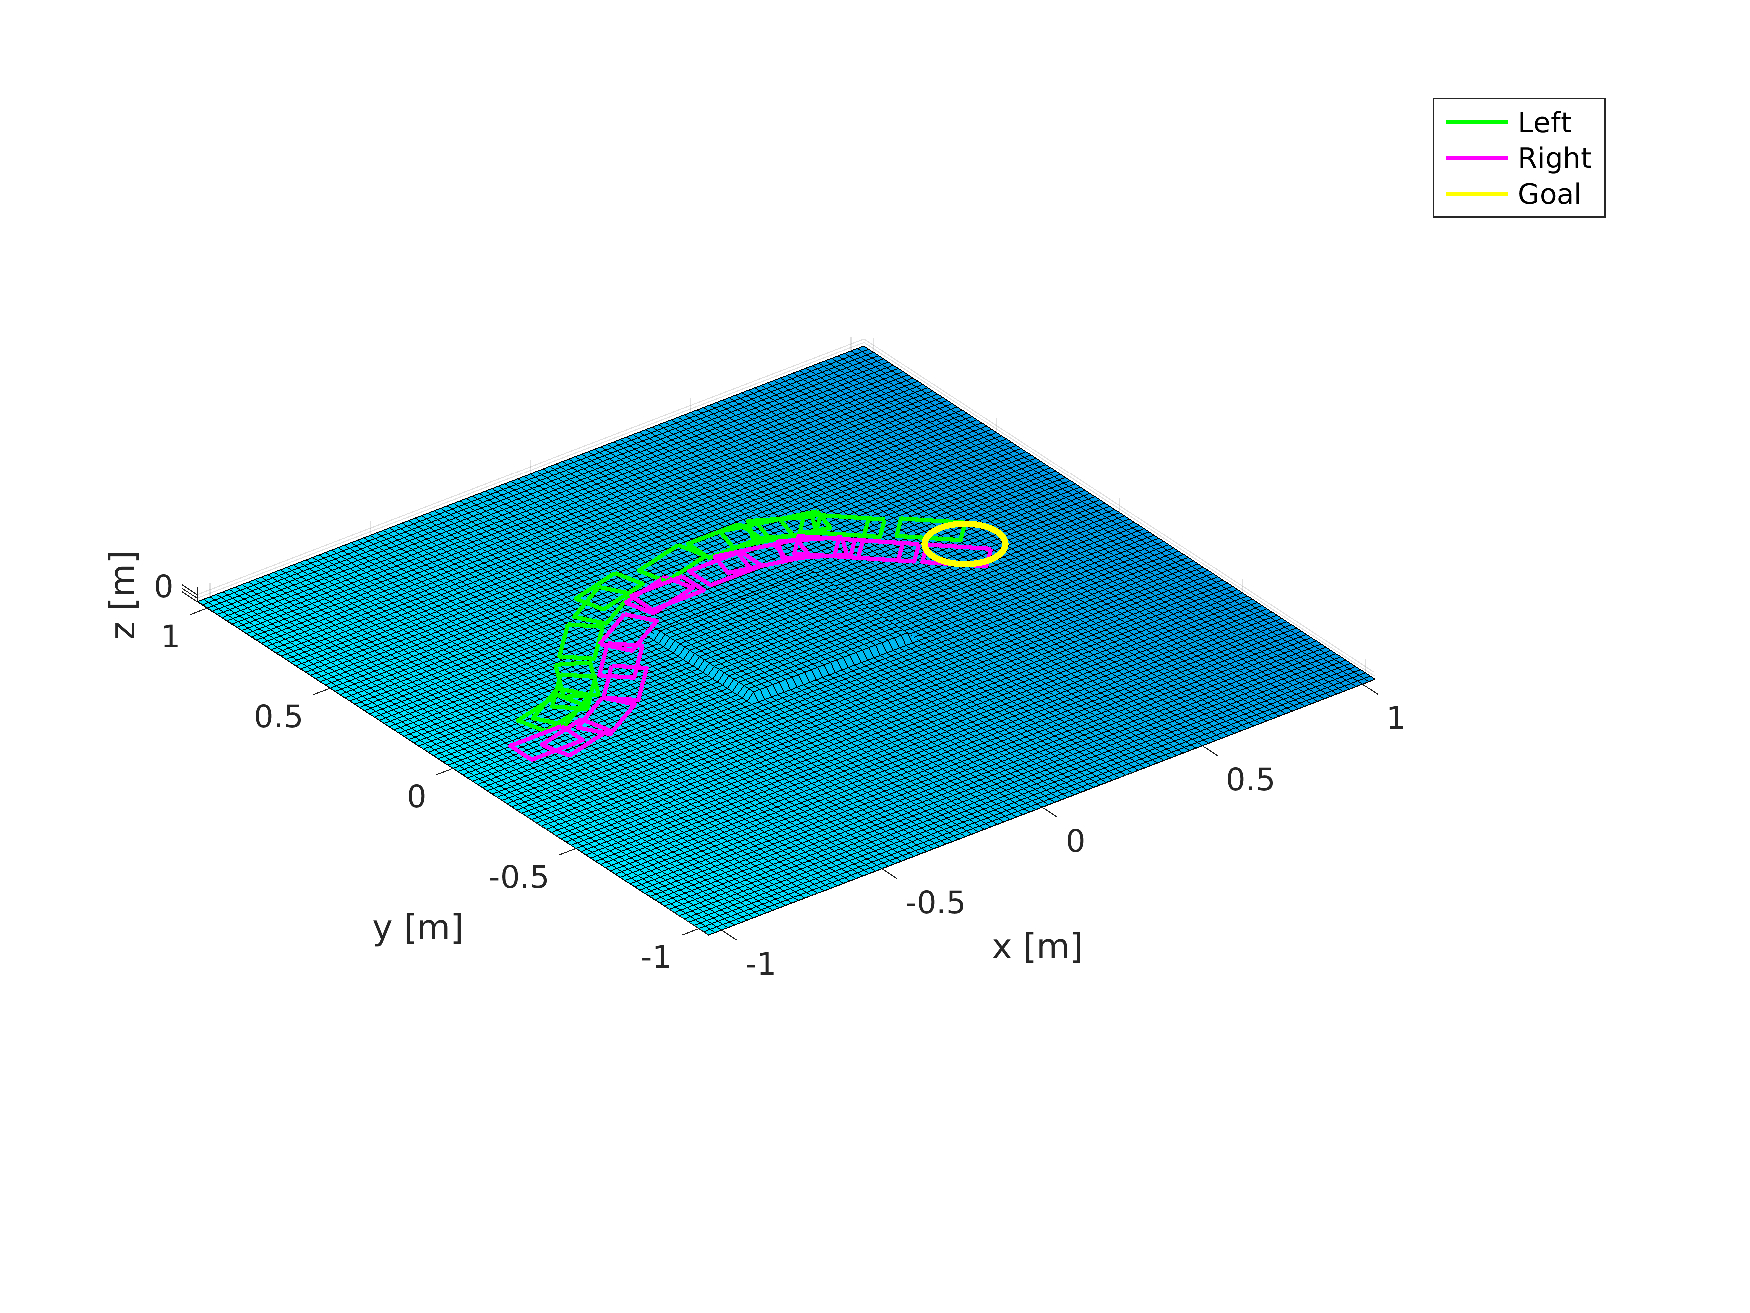
\includegraphics[width=0.95\textwidth]
        {figures/experiments/obstacle-avoidance/footstep-plan.pdf}
    \caption{Footstep plan generated for the scenario ``Obstacle Avoidance''.}
    \label{fig:experiments:obstacle-avoidance:footstep-plan}
\end{figure}
\begin{figure}
    \centering
    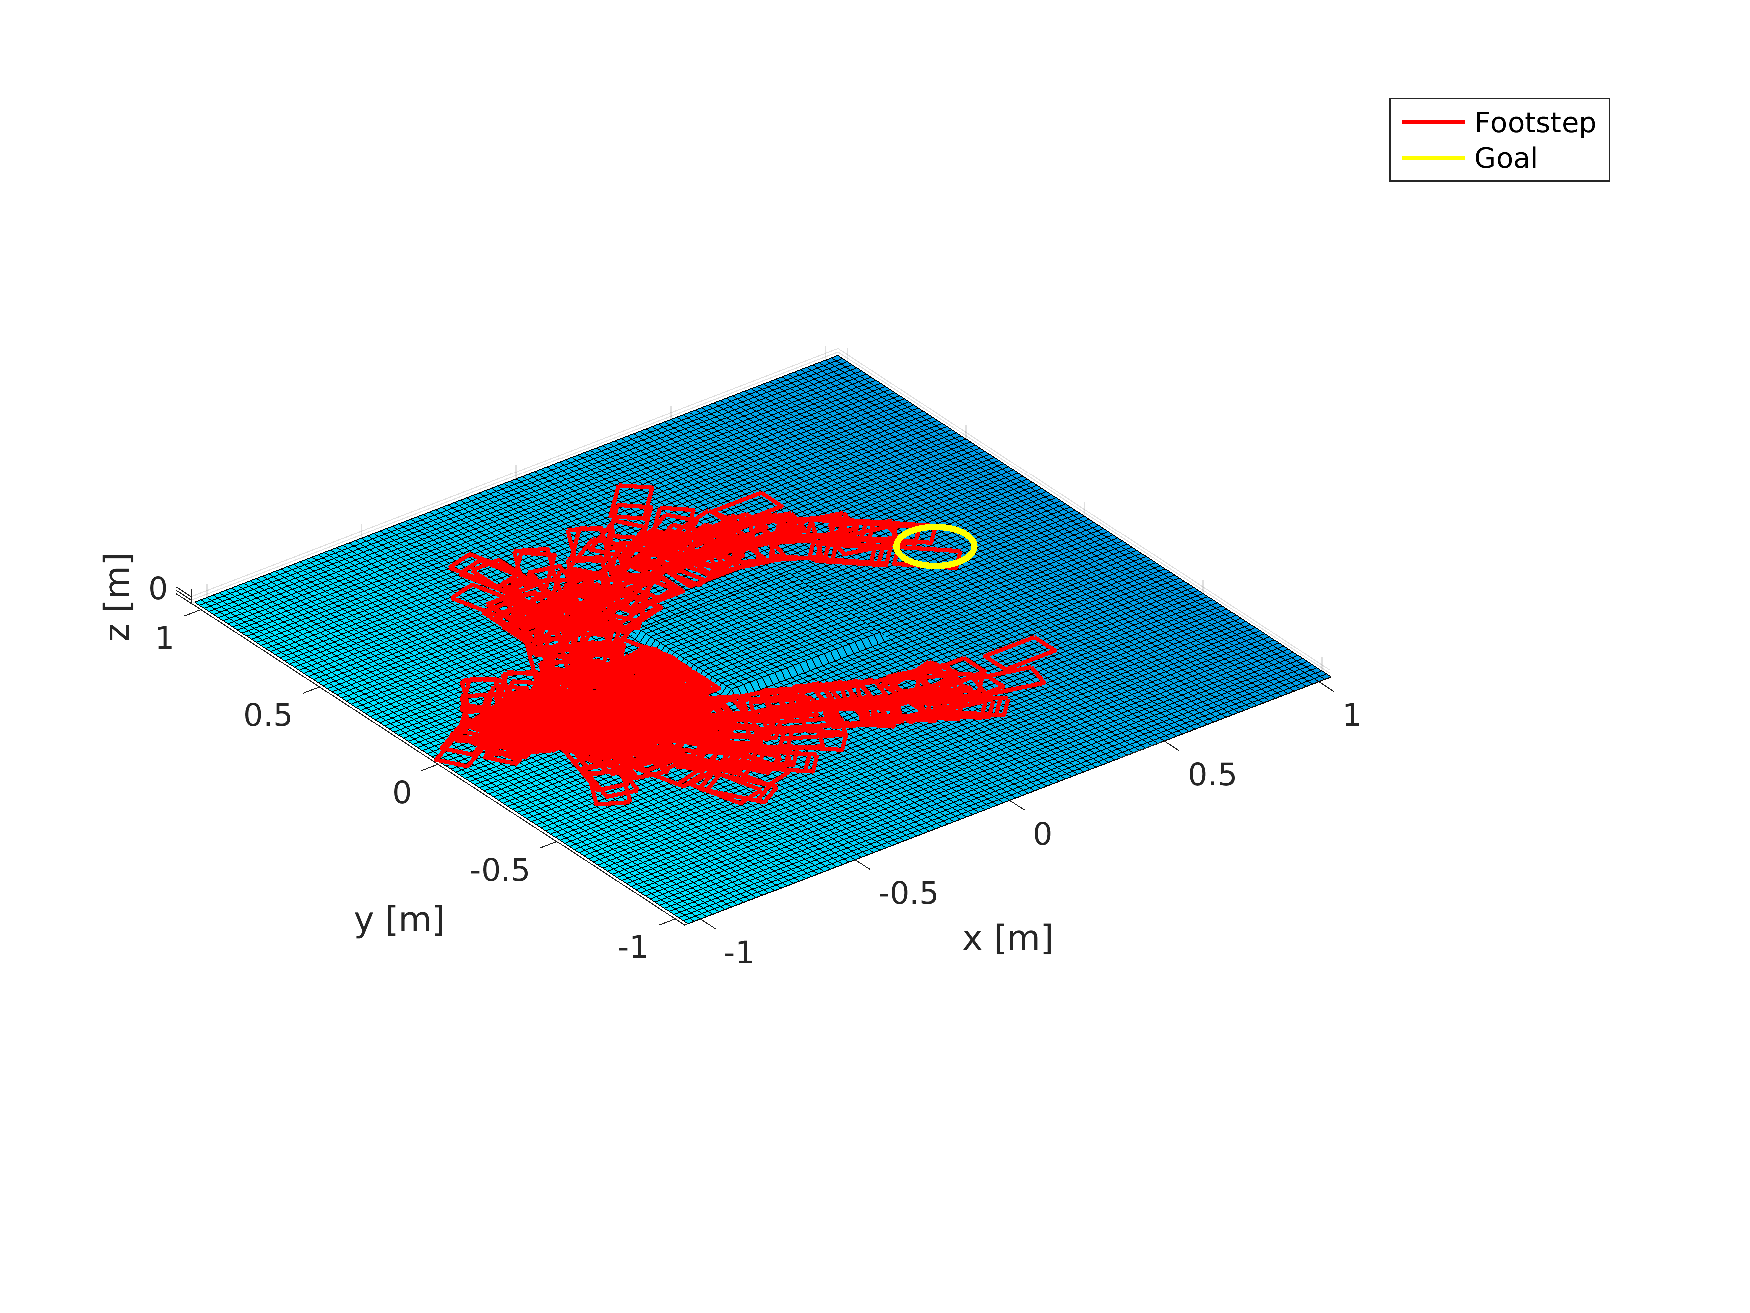
\includegraphics[width=0.95\textwidth]
        {figures/experiments/obstacle-avoidance/rrt-tree.pdf}
    \caption{Tree generated for the scenario ``Obstacle Avoidance''.}
    \label{fig:experiments:obstacle-avoidance:rrt-tree}
\end{figure}

\section{Stair Climbing in Unknown Environment}
Stair climbing (unknown environment). Planner + \texttt{elevation\_mapping}.
\begin{figure}
    \centering
    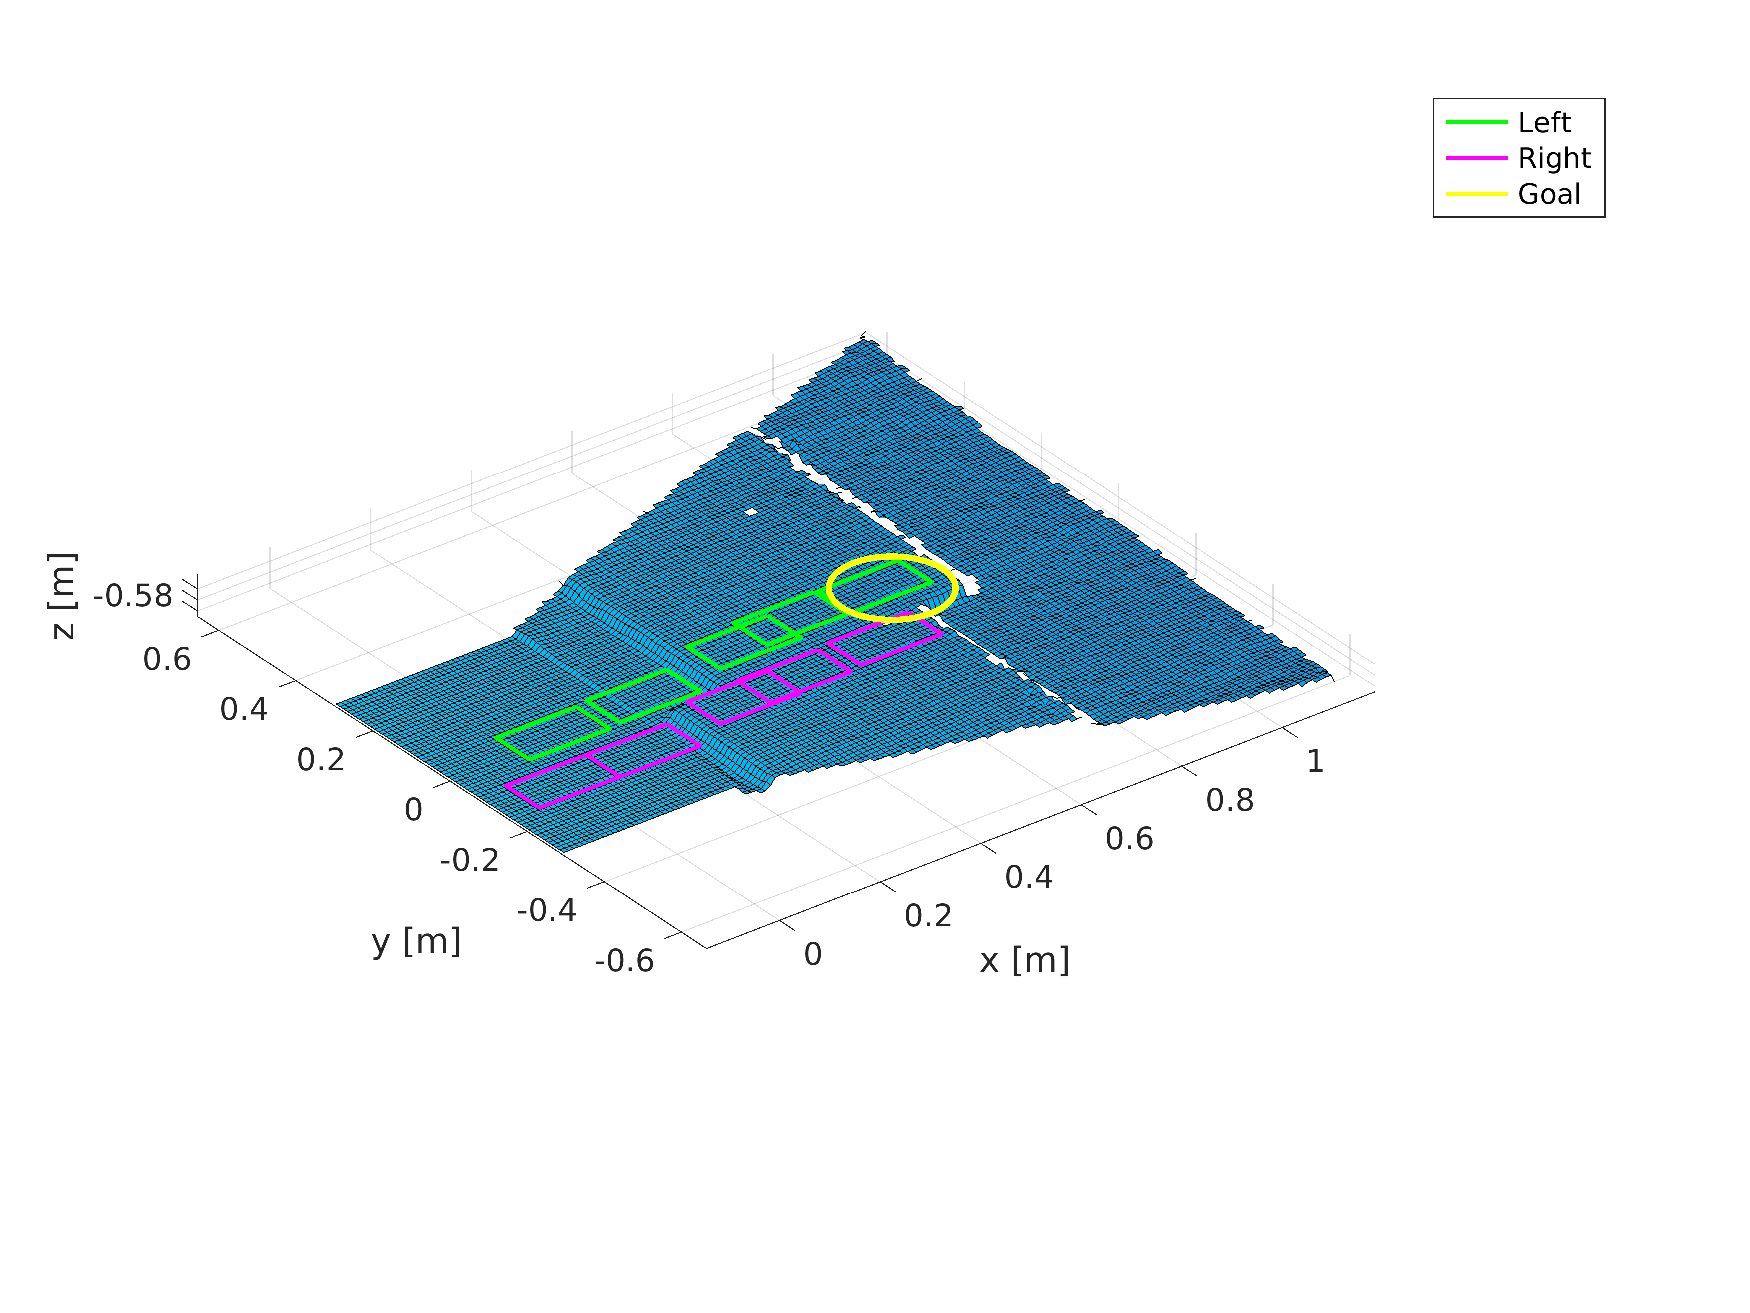
\includegraphics[width=0.95\textwidth]
        {figures/experiments/unknown-env/footstep-plan.pdf}
    \caption{Footstep plan generated for the scenario ``Stair Climbing in 
        Unknown Environments''.}
    \label{fig:experiments:unknown-env:footstep-plan}
\end{figure}
\begin{figure}
    \centering
    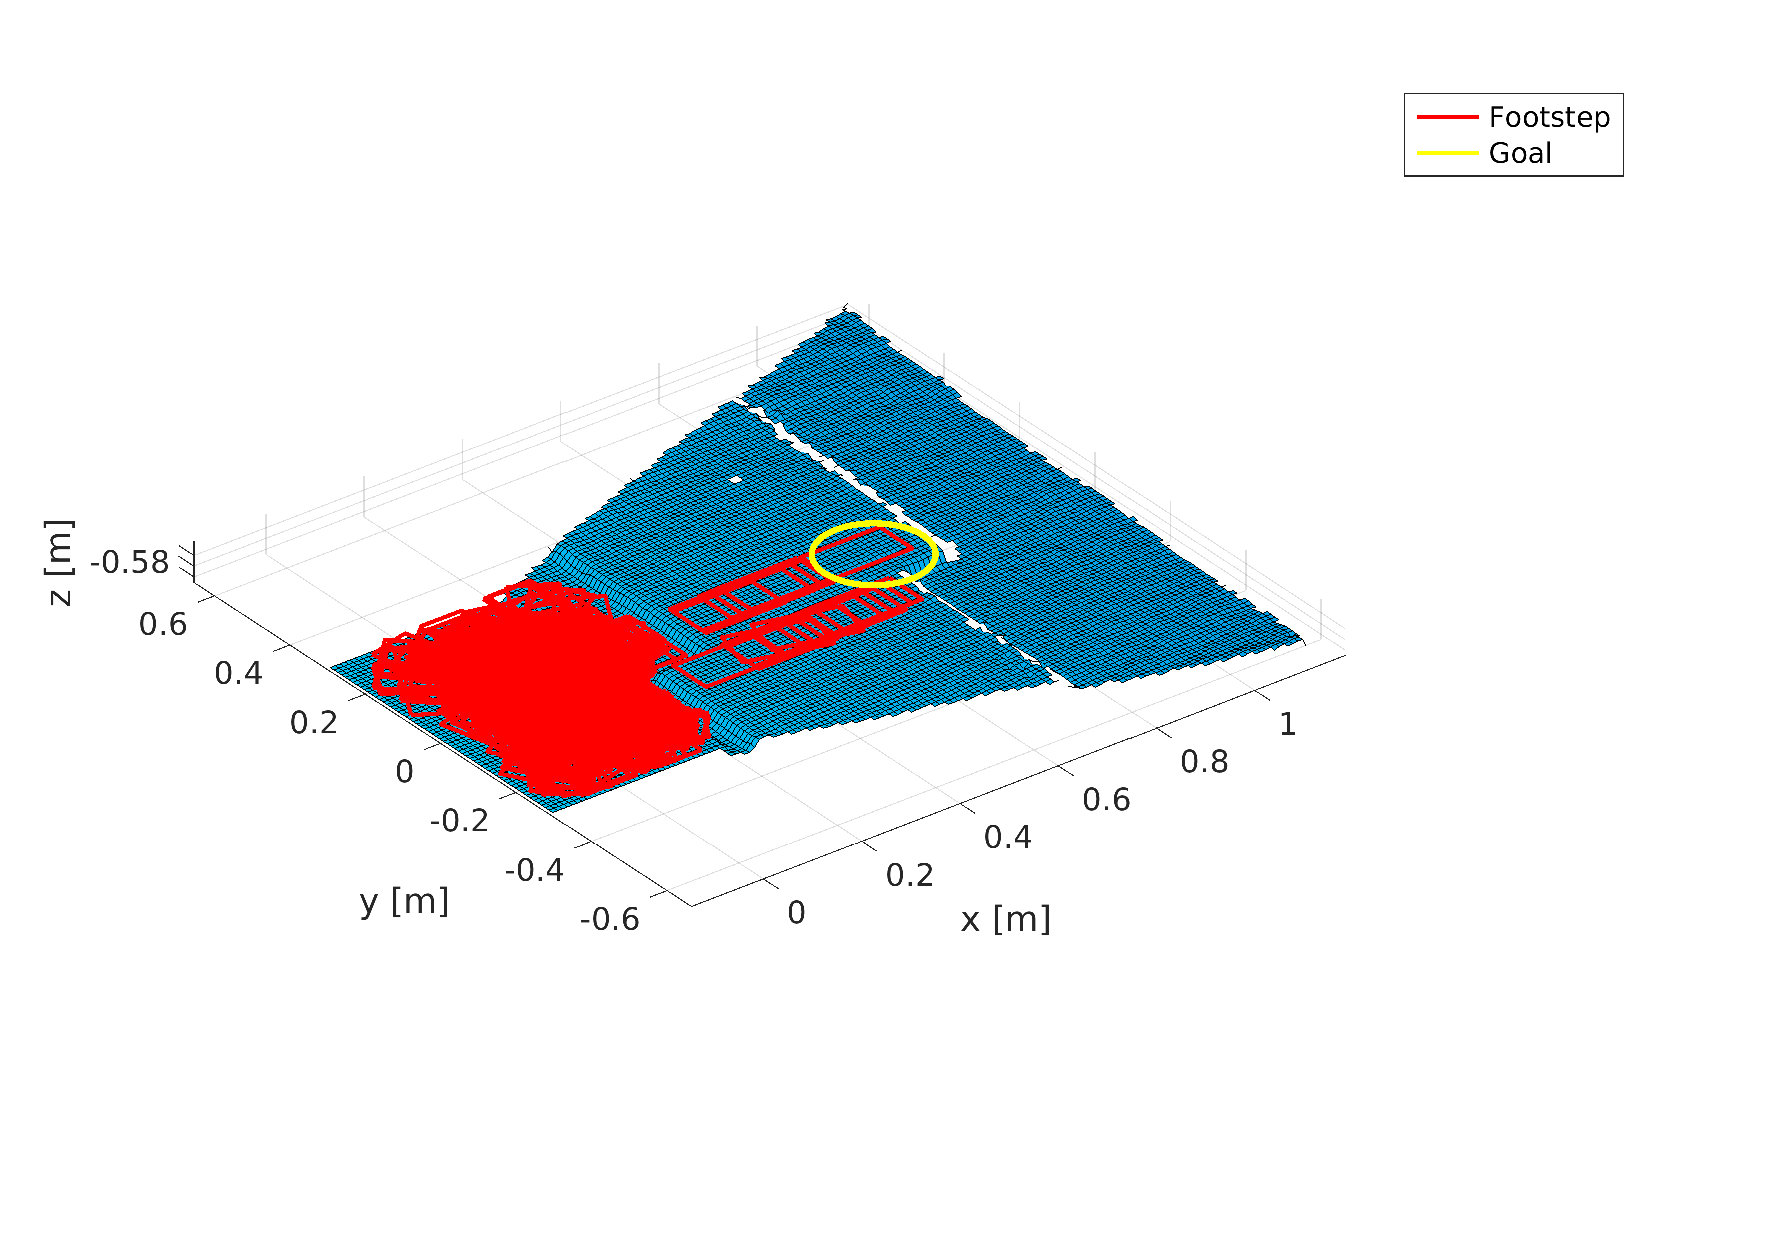
\includegraphics[width=0.95\textwidth]
        {figures/experiments/unknown-env/rrt-tree.pdf}
    \caption{Tree generated for the scenario ``Stair Climbing in 
        Unknown Environments''.}
    \label{fig:experiments:unknown-env:rrt-tree}
\end{figure}


\chapter{Conclusion}
\label{ch:conclusion}
\section{Results}
This thesis presents an architecture that integrates mapping, planning and 
control to generate humanoid gaits in \textit{World of Stairs} unknown 
environments. The use of \texttt{elevation\_mapping}
\cite{Fankhauser2018ProbabilisticTerrainMapping} together with a depth
sensor allows the robot to represent the surrouding environment as a map that
can be used by a RRT-based footstep planning module \cite{ECC19}
to generate a sequence
of footsteps. The Variable-Height CoM IS-MPC \cite{SYROCO18} 
has been implemented on NAO
humanoid robot upon the BHuman framework and the whole architecture has been
tested on multiple scenarios.

\section{Future Works}
The current architecture does not include a localization module, limiting the
potentialities of the robot. Localizing the robot inside the environment would,
in fact, provide a precise configuration of the humanoid, enabling 
\texttt{elevation\_mapping} to continuously build the map during locomotion.
A possible extension could be to develop such module using a Kalman filter
\cite{Bloesch2013StateEstimationLeggedRobots} or a factor graph
\cite{Wisth2019PreintegratedVelocityBiasEstimation}.
Another possible extension of this work could be that of developing a replanning
phase \cite{Griffin2019FootstepPlanningRoughTerrain}, allowing the robot to
work in dynamic environments. The combination of these two could give even
more autonomy to humanoid robots, further advancing current technology and
allowing their introduction into our society.



\backmatter
% bibliography
\cleardoublepage
\phantomsection
%\bibliographystyle{sapthesis} % BibTeX style
\bibliographystyle{unsrt}
\bibliography{bibliography} % BibTeX database without .bib extension

\end{document}
